	%\setcounter{section}{7}  %PAGE1
	\section{ВАРИАЦИОННОЕ ИСЧИСЛЕНИЕ}
	\subsection{Примеры задач с бесконечным числом степеней свободы}

	Всюду выше рассматривались оптимизационные задачи в конечномерном пространстве. Это значит, что целевые функции этих задач являлись функциями конечного числа n переменных, которые удовлетворяли некоторым ограничениям. Однако сравнительно давно появились оптимизационные задачи, в которых разыскиваемую «точку оптимума» нельзя охарактеризовать конечным числом параметров (степеней свободы). Подобные задачи и составляют содержание вариационного исчисления, основанного в XVIII веке Л. Эйлером и Ж. Лагранжем, и значительно развитого в XIX веке в трудах ряда выдающихся математиков. В настоящее время вариационное исчисление превратилось в один из важнейших разделов теоретической и прикладной математики. Приведем ряд примеров задач, сыгравших важную роль в зарождении вариационного исчисления.

	\primer{ Исторически первой задачей, известной из глубокой древности и отнесенной впоследствии к задачам вариационного исчисления, явилась так называемая задача Дидо. Согласно легенде Дидо – царица одного из государств Древней Греции, преследуемая царем соседнего государства, бежала в Северную Африку и попросила у местного населения участок земли, который можно охватить шкурой вола. Получив согласие на столь ничтожную просьбу, она на глазах изумленных зрителей разрезала шкуру на тонкие ремешки и, связав их друг с другом, охватила полученной нитью довольно большой по тем временам участок. Развернув на нем строительство, она основала на этом участке знаменитый в древности город Карфаген.

	Античные ученые заинтересовались математической стороной этой легенды: если нить уже связана, как расположить ее, чтобы охватить участок с площадью, наибольшей из возможных. В этой задаче требуется найти кривую заданной длины, которая охватывает наибольшую площадь. Она имеет ряд вариантов, и впоследствии получила название изопериметрической задачи. Уже в древности было обнаружено, что искомой формой нити здесь является дуга окружности (рис. \ref{picture_8_1}). Один из вариантов задачи состоит в максимизации интеграла $$\textstyle S = \int\limits_a^b y(x)\,dx$$ ($y=y(x)$–уравнение сухопутной границы участка), при заданном значении длины нити, то есть интеграла

	%PAGE2
	\newpage
	\noindent
	$$\textstyle L = \int\limits_a^b \sqrt{1+y'^2}\,dx$$
	и заданных краевых условиях $y(a)=y(b)=0$.
	\begin{figure}[!htb]
   \begin{minipage}{0.48\textwidth}
     \centering
     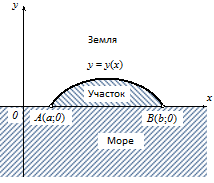
\includegraphics{pictures/picturefile_8_1.png}
     \caption{}\label{picture_8_1}
   \end{minipage}\hfill
   \begin {minipage}{0.48\textwidth}
     \centering
     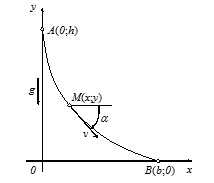
\includegraphics{pictures/picturefile_8_2.png}
     \caption{}\label{picture_8_2}
   \end{minipage}
\end{figure}
}

\primer{ Другой знаменитой задачей, приведшей к созданию методов вариационного исчисления, явилась задача о брахистохроне, предложенная И. Бернулли в $1696$ году. Она состоит в следующем. Рассматривается материальная точка $M$, которая скатывается под действием силы тяжести без трения вдоль некоторой линии $y(x)$ из заданной точки $A$ в заданную точку $B$ (рис. \ref{picture_8_2}), затрачивая на это время $T$. Требуется так выбрать путь скатывания $y(x)$, чтобы время $T$ было минимальным из возможных. Перейти к чисто математической задаче здесь помогает закон сохранения энергии
	\[gm(h-y)=\frac{mv^2}{2}\text{, откуда } v = \sqrt{2g(h - y)}\text{.}\]

	Далее
	\[\frac{dx}{dt}=v\cos\alpha=\frac{\sqrt{2g(h-y)}}{\sqrt{1+y'^2}}\text{, то
	есть } dt=\sqrt{\frac{1+y'^2}{2g(h-y)}}dx\text{.}\]

	Поэтому
	\[\textstyle T=\int dt=\int\limits_0^b \sqrt{\frac{1+y'^2}{2g(h-y)}}\,dx\text{.}\]

	Таким образом, речь идет о подборе функции $y(x)$, минимизирующей значение интеграла $T$. При этом функция $y(x)$ должна дополнительно удовлетворять граничным условиям $y(0)=h$,

	%PAGE3
	\newpage
	\noindent
	$y(b)=0$.
\vspace*{-\baselineskip}
	\begin{figure}[h]
		\center{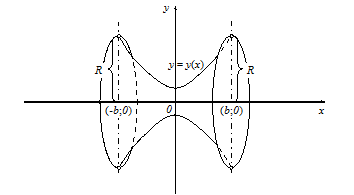
\includegraphics{pictures/picturefile_8_3.png}}
		\caption{}
		\label{picture_8_3}
	\end{figure}
\vspace*{-\baselineskip}
}

	\primer{ Рассмотрим также задачу о форме равновесия мыльной пленки, натянутой на два кольца, насаженных на общую ось (рис. \ref{picture_8_3}). Для простоты будем считать кольца одинаковыми, а ось, соединяющую их центры, перпендикулярной параллельным плоскостям колец. Примем также естественную гипотезу, что поверхность пленки имеет форму поверхности вращения, которая получается вращением вокруг оси центров колец кривой, заданной уравнением $y=y(x)$. Если пренебречь весом пленки, то из теории поверхностного натяжения будет следовать, что пленка должна иметь минимально возможную площадь. Математически задача сведется к минимизации интеграла
	\[\textstyle \sum=\int\limits_{-b}^b y\sqrt{1+y'^2}\, dx\text{,}\]
	равного площади поверхности вращения, при граничных условиях
	\[y(-b)=y(b)=R\text{.}\]
	Таким образом, и в этом примере речь идет о подборе функции $y(x)$, минимизирующей значение интеграла $\sum$.

	Нетрудно увидеть в приведенных примерах общие черты. Прежде всего, в этих примерах появляются задачи на экстремум – минимум или максимум. В предыдущих главах мы имели дело с задачами на экстремум функций $z = f(x_1, x_2, \dots, x_n) $ от n переменных. Искомым там был набор значений $x_1 ,x_2, \dots, x_n$. Такую задачу обычно называют задачей с $n$ степенями свободы. В задачах же этого параграфа искомой является линия, или, на аналитическом языке, функция, от которой требуется только, чтобы она удовлетворяла заданным граничным условиям. Но при произвольном выборе такой функции имеется

	%PAGE4
	\newpage
	\noindent
бесконечное число степеней свободы, поскольку произвольную линию или функцию нельзя задать конечным набором параметров. Таким образом, рассмотренные примеры действительно можно отнести к оптимизационным задачам с бесконечным числом степеней свободы. }
	\subsection{Понятие функционального пространства и функционала в нем. Локальный экстремум функционала. Общая схема исследования функционала на экстремум}

{\bf Примеры функционалов.} Основные понятия вариационного исчисления во многом аналогичны понятиям теории экстремумов функций конечного числа аргументов, где основную роль играет целевая функция со своей областью определения. Если, например, в интеграл $\sum$ примера 8.3 вместо $y(x)$ подставить любую конкретную функцию, заданную на сегменте	$[-b, b]$ и удовлетворяющую краевым условиям $y(-b)=y(b)=R$, то он примет определенное числовое значение. {\it Такой закон соответствия, который каждой функции из некоторого класса функций ставит в соответствие число, называется функционалом}. Задача примера 8.3 состоит в подборе функции $y(x)$ для которой функционал $\sum$ принимает минимальное значение. Задача примера 8.1 является задачей на максимум функционала $S$. Вариационное исчисление изучает экстремумы функционалов.

Отметим, что функционал определяется как самим законом, сопоставляющим функции число, так и классом функций на котором он определен. Например, функционал $\displaystyle I = I\{y\} = \int\limits_0^2 y^2(x)\,dx$ можно считать определенным на функциях, заданных при $0\leq x\leq 2$,принимающих там конечные значения (или даже бесконечные, если интеграл окажется сходящимся). Но его можно также определить на гладких функциях, удовлетворяющих граничным условиям $y(0)=y(2)=0$. И это будет уже другой функционал. Можно сказать, что {\it функционал – это функция, у которой независимой переменной $y(x)$ служат обычные функции из некоторого класса функций, а значениями зависимой переменной $I\{y(x)\}$ служат числа.}

{\bf Нормированное векторное пространство. Общая точка зрения на функционал.} . В теории экстремумов функций конечного числа переменных область определения функции является множеством в векторном пространстве $R^n$. Для функционалов область определения является множеством в {\it линейном векторном пространстве функций}.

	%PAGE5
	\newpage
	\noindent
	{\it Линейное векторное пространство} $H$ - это совокупность элементов $u, v, ...,$ называемых векторами, для которых определены {\it линейные операции} (сложение $u+v$ двух векторов $u, v$ и умножение $\alpha u$ вектора $u$ на скаляр $\alpha$), подчиняющиеся обычным правилам линейной алгебры. Ниже скаляры предполагаются {\it вещественными числами}. Обычно нулевой вектор обозначается символом {\bf 0}, тем же, что и нулевой скаляр.

Векторы $u_1, u_2, ..., u_n$ называются {\it линейно независимыми}, если их линейная комбинация $\alpha_1 u_1+...+\alpha_n u_n$ равна нулю только в том случае, когда $\alpha_1=...=\alpha_n=0$; в противном случае эта система векторов называется {\it линейно зависимой}. Под {\it размерностью} $dimH$ векторного пространства $H$ понимают наибольшее число линейно независимых векторов в нем. Если такого наибольшего числа не существует, полагают, что $dimH=\infty$ и векторное пространство называют {\it бесконечномерным}. В противном случае говорят о {\it конечномерном} векторном пространстве.

Подмножество $M\subset H$ называется {\it линейным подпространством} или {\it однородным линейным многообразием} в $H$, если $M$ само является векторным пространством относительно линейных операций в $H$. Размерность $M$ не превосходит размерности пространства $H$.

Обычно для каждого вектора $u\in H$ определено число $\| u \| $, которое называется нормой вектора $u$. Норма обладает следующими свойствами:
\begin{flushleft}
	$\mspace{72mu}1)\| u \|\ge0 $

	$\mspace{72mu}2)\| u \|=0 $ тогда и только тогда, когда $u={\bf 0}$.

	$\mspace{72mu}3)\| \alpha u \|= |\alpha | \| u \|$

	$\mspace{72mu}4)\| u+v \|\le \| u \|+\| v \| $
\end{flushleft}

Линейное векторное пространство $H$, в котором определена норма, удовлетворяющая условиям 1)-4), называется {\it нормированным векторным пространством}. В вариационном исчислении наиболее употребительными являются следующие функциональные нормированные векторные пространства.

	1. Пространство $C[a, b]$ функций $u(x)$, заданных и непрерывных на конечном отрезке $a\le x \le b$ с нормой
$$\|u\|= \max_{a\le x\le b}|u(x)|.$$
	\vspace*{-\baselineskip}

	2. Пространство $C_1[a, b]$ функций $u(x)$, заданных и непрерывных при $a\le x \le b$ вместе со своей производной, с нормой

	%PAGE6
	\newpage
	\noindent
	$$\|u\|= \max_{a\le x\le b}|u(x)| + \max_{a\le x\le b}|u'(x)|.$$
	Аналогично вводится пространство $C_n[a,b]$ при $n=2,3,4,\dots$

	3. Гильбертово пространство $L_2[a,b]$ функций, заданных при \\* $a\le x\le b$,
	не обязательно непрерывных, для которых норма
	$$\textstyle \|u\|=\sqrt{\int\limits_a^b |u(x)|^2, dx}$$
	принимает конечное значение. Это означает, что функция $u(x)\in L_2[a,b]$
	должна быть {\it квадратично суммируемой.}

	Легко проверить, что каждая из перечисленных выше норм удовлетворяет условиям 1)-4).

	Всякая функция из $C_1[a, b]$ принадлежит $C[a, b]$, а всякая функция из $C[a, b]$ принадлежит $L_2[a, b]$. Тем не менее, $C_1[a, b]$ нельзя считать подпространством $C[a, b]$, поскольку эти пространства рассматриваются неотделимо от своих норм, а нормы в $C_1$ и $C$ различны.

	В нормированном пространстве вводится понятие расстояния $\rho$ между любыми элементами $u, v$ по формуле $\rho (u, v)=\|u-v\|$. Для пространств, состоящих из функций, это расстояние является уклонением функций друг от друга, причем каждая из норм дает свое измерение этого уклонения.

	Элементы нормированного пространства не обязательно являются функциями. Поэтому на функционал можно смотреть с абстрактной точки зрения, {\it как на функцию $I\{u\}$, определенную на некотором множестве $N(I)\subset H$}. Дадим абстрактное определение экстремума функционала. При этом $\epsilon$ - окрестностью $U_\epsilon (u)$ точки
	$u\in H$ будем называть множество элементов $v\in H$, удовлетворяющих неравенству
	$\|u-v\| < \epsilon$ при некотором $\epsilon > 0$.

	\opredelenie{Элемент $U_0\in N(I)$ называется точкой локального минимума (максимума) функционала $I\{u\}$, если найдется такая окрестность $U_\epsilon (u_0)$, что для всех
$u\in U_\epsilon (u_0)\cap N(I)$ выполнено неравенство $I\{u\}\ge I\{u_0\}$
($I\{u\}\le I\{u_0\}$). Элемент $u_0$ естественно назвать локальным экстремумом функционала $I\{u\}$.}

	Отметим, что в последнем определении, по сути, требуется, чтобы соответствующие неравенства выполнялись для всех элементов $u\in N(I)$ достаточно близких к $u_0$. Для функциональных пространств достаточная близость означает достаточно малое уклонение функции $u(x)$ от функции $u_0(x)$. Но эти уклонения могут измеряться различными способами в зависимости от того, какое функциональное пространство

	%PAGE7
	\newpage
	\noindent
	(норму) взять за основу. В соответствии с этим рассматривают различные типы экстремумов функционалов в функциональных пространствах. В дальнейшем мы будем чаще всего исследовать функционалы, которые естественно рассматривать либо в $C_1[a, b]$, либо в $C[a, b]$. В первом случае функцию $u_0(x)$ (элемент $u_0$) будем называть {\it слабым}, а во втором – {\it сильным экстремумом} функционала. При этом, сильный экстремум всегда будет также и слабым, но обратное не обязательно. Например, для функционала $I\{u\} = \int\limits_0^1 \sqrt[4]{1+u'^2} dx$, определенного на гладких функциях $u(x)$, удовлетворяющих краевым условиям $u(0)=0$, $u(1)=1$, функция
	$u_0(x)=x$ доставляет слабый минимум. В то же время сильного минимума эта функция не дает.

	Для изложения абстрактной схемы исследования функционала на экстремум нам понадобиться следующее

	\opredelenie{Функционал $J\{u\}$ в линейном векторном пространстве $H$ называется линейным, если его область определения $N(J)\subseteq H$ является линейным подпространством в $H$, и он обладает свойствами аддитивности: $J\{u+v\}=J\{u\}+J\{v\}$ и однородности: $J\{Cu\}=CJ\{u\}$, где $u, v\in N(J)$, $C=const$.}

	{\bf Вариация функционала. Необходимые условия экстремума}.
	Предположим, что первоначально мы имели элемент $u_0$, а затем перешли к элементу $u=u_0+\delta u$. Здесь элемент $\delta u$ (символ нужно понимать как единый) принято называть вариацией элемента $u_0$ при условии, что вновь полученный элемент $u\in N(I)$. В остальном вариация $\delta u$ считается произвольной и, обычно, малой по норме.
	Отметим, что вариация $\delta u$ полностью аналогична конечномерному вектору приращений аргументов в теории экстремумов функций нескольких аргументов. Действуя по аналогии, рассмотрим приращение функционала $\Delta I=I\{u_0+\delta u\}-I\{u_0\}$. Ниже мы будем предполагать, что функционал $I\{u\}$ обладает следующим свойством: для любого элемента $u_0\in N(I)$ приращение функционала $\Delta I$ является суммой двух слагаемых
	\begin{equation}
	\label{equation_8_1}
         \Delta I=J\{u_0, \delta u\}+R_1\{u_0, \delta u\}\text{,}
    	\end{equation}
    первое из которых при фиксированном $u_0$ является линейным функционалом относительно $\delta u$, а второе удовлетворяет условию
   \begin{equation}
	\label{equation_8_2}
    	|R_1\{u_0, \delta u\}|=o(\|\delta u\|)\text{, при }\|\delta u\|\to 0.
   \end{equation}

	Отметим, что свойство (\ref{equation_8_1}), (\ref{equation_8_2}) аналогично свойству дифференцируемости функций одного или нескольких аргументов, и, если это свойство имеет место, совершенно аналогично можно

	%PAGE8
	\newpage
	\noindent
	установить необходимые условия экстремума функционала. Отметим, что слагаемое $\delta I\{u_0, \delta u\}=J\{u_0, \delta u\}$ в (\ref{equation_8_1}) называют вариацией функционала в данной точке $u_0$. Этот линейный по $\delta u$ функционал можно считать определенным во всем пространстве $H$, хотя в конкретных случаях $\delta u$ может принадлежать более узкому, чем $H$ подпространству. Понятие вариации $\delta I\{u_0, \delta u\}$ полностью аналогично понятию дифференциала функции нескольких аргументов.

	\teorema{\it Если элемент $u_0$ является точкой экстремума функционала $I\{u\}$, то при любой возможной вариации $\delta u$ аргумента вариация функционала при данном $u_0$ равна нулю
		$$\delta I\{u_0, \delta u\}=0\text{.}$$}

	\vspace*{-\baselineskip}
	Д\,о\,к\,а\,з\,а\,т\,е\,л\,ь\,с\,т\,в\,о. Предположим противное, то есть что найдется такая возможная вариация $\delta u$, при которой $\delta I\{u_0, \delta u\}>0$. Для определенности будем считать, что $\delta I\{u_0, \delta u\}>0$. При некоторой константе $t$ рассмотрим приращение
	\begin{gather}
	\Delta I=I\{u_0+t\delta u\}-I\{u_0\}=\delta I\{u_0, t\delta u\}+R_1\{u_0, t\delta u\}=t(\delta I\{u_0, \delta u\}+\notag\\
	+t^{-1}R_1\{u_0,t\delta u\})\text{.}\notag
	\end{gather}

	В силу условия (\ref{equation_8_2}) при $t\to 0$ второе слагаемое в последних скобках стремиться к нулю, и эти скобки положительны при достаточно малых $|t|$. Это значит, что знак приращения $\Delta I$ совпадает со знаком $t$ и может принимать как положительные, так и отрицательные значения. Но поскольку $u_0$ по условию является экстремумом функционала приращение $\Delta I$ при достаточно малых $|t|$ не должно изменять знак. Пришли к противоречию. Теорема доказана.

	{\bf Вариации функционала высших порядков. Достаточные условия экстремума.} Еще раз подчеркнем глубокую аналогию между дифференциальным и вариационным исчислениями. Ее наличие позволяет ожидать, что при переходе к достаточным условиям экстремума функционала появиться понятие, играющее в этом вопросе ту же роль, что и дифференциал второго порядка при исследовании экстремума функций нескольких аргументов. Этим понятием является вторая вариация.

	Для многих типов функционалов справедлива формула
	\begin{gather}
		\Delta I=I\{u_0+\delta u\}-I\{u_0\}=\delta I\{u_0,\delta u\}+(\frac{1}{2!})\delta^2 I\{u_0,\delta u\}+\dots+\notag\\
		+(\frac{1}{n!})\delta^n I\{u_0,\delta u\}+R_n\{u_0,\delta u\}\text{,}\notag
	\end{gather}
	совершенно аналогичная формуле Тейлора для функций конечного числа аргументов. Здесь $\delta^2 I\{u_0,\delta u\}$, $\delta^3 I\{u_0,\delta u\}$,$\dots$,$\delta^n I\{u_0, \delta u\}$ -- {\it вариации функционала соответственно второго, третьего и т. д. порядков.} ({\it кратко –- вторая, третья и т. д. вариации}). Они являются

	%PAGE9
	\newpage
	\noindent
	функционалами относительно $\delta u$ уже не линейными, однако обладающими свойством однородности соответствующей степени
	$$\delta^n I\{u_0, k\delta u\}=k^n \delta^n I\{u_0, \delta u\}, k=const.$$
	Это означает, что члены $\delta^n I\{u_0, \delta u\}$ при $n=2, 3,\text{ } \dots$имеют последовательно второй, третий и т. д. порядок малости относительно $\|du\|$. Остаточный член $R_n\{u_0,\delta u\}$ обладает свойством
	\begin{equation}
		\label{equation_8_3}
		|R_n\{u_0, \delta u\}|\le C\|\delta u\|^{n+1}\text{.}
	\end{equation}
	Элемент $u_0\in N(I)$, удовлетворяющий при всех возможных $\delta u$ условию ($\delta I\{u_0,\delta u\}=0$) обычно называют {\it стационарным элементом функционала} $I\{u\}$. Всюду ниже мы предполагаем справедливость аналога формулы Тейлора при $n=2$. Характер стационарного элемента можно выяснить с помощью {\it достаточных условий экстремума функционала}

	\teorema{{\it Пусть элемент $u_0$ является стационарным элементом функционала $I\{u\}$. Тогда справедливы следующие утверждения.

		$1^0$. Если при любой возможной вариации $\delta u$ вторая вариация функционала удовлетворяет неравенству $\delta^2 I\{u_0, \delta u\}\geq m\|\delta u\|^2$ при некоторой константе $m>0$, то стационарный элемент u0 является точкой локального минимума функционала.

		$2^0$. Если при любой возможной вариации $\delta u$ вторая вариация функционала удовлетворяет неравенству $\delta^2 I\{u_0, \delta u\}\le {-m}\|\delta u\|^2$ при некоторой константе $m>0$, то стационарный элемент $u_0$ является точкой локального максимума функционала.

		$3^0$. Если при различных возможных вариациях $\delta u$ вторая вариация функционала $\delta^2 I\{u_0, \delta u\}$ принимает значения разных знаков, то стационарный элемент $u_0$ не является точкой локального экстремума функционала (функционал имеет при $u=u_0$ минимакс).}}

	Д\,о\,к\,а\,з\,а\,т\,е\,л\,ь\,с\,т\,в\,о. Запишем приращение $\Delta I=I\{u_0+\delta u\}-I\{u_0\}$ с помощью аналога формулы Тейлора с $n=2$, учитывая, что $u_0$ - стационарный элемент функционала $I\{u\}$. Получим
	$$\Delta I=I\{u_0+\delta u\}-I\{u_0\}=\frac{1}{2}\delta^2 I\{u_0,\delta u\}+R_2\{u_0,\delta u\}$$

	При условиях $1^0$ с учетом свойства (\ref{equation_8_3}) получаем оценку $\Delta I\geq \frac{m}{2}\|\delta u\|^2-C\|\delta u\|^3$, из которой следует положительность $\Delta I$ при $\|\delta u\|<\frac{m}{2C}$. То есть стационарный элемент $u_0$ является точкой локального минимума функционала, и пункт $1^0$ доказан. При условиях $2^0$ точно также получаем оценку $\Delta I\le {-\frac{m}{2}}\|\delta u\|^2+C\|\delta u\|^3$, из которой следует отрицательность $\Delta I$ при $\|\delta u\|<\frac{m}{2C}$. Тем самым и пункт $2^0$ тоже доказан.

	%PAGE10
	\newpage
	Для доказательства пункта $3^0$ теоремы достаточно доказать, что при его условиях в любой окрестности стационарного элемента $u_0$ найдутся элементы $u_1$, $u_2$, для которых выполнены неравенства $I\{u_1\}>I\{u_0\}$ и $I\{u_2\}<I\{u_0\}$. По условию пункта $3^0$ найдутся такие $(\delta u)_1$ и $(\delta u)_2$, что $\delta^2 I\{u_0,(\delta u)_1\}>0$ и $\delta^2 I\{u_0,(\delta u)_2\}<0$. Будем искать упомянутые $u_1$, $u_2$ в виде $u_1=u_0+t(\delta u)_1$, $u_2=u_0+t(\delta u)_2$, где $t$ –некоторое число. Тогда справедливы следующие оценки.
	\begin{gather}
	\scalebox{.9}{$I\{u_0+t(\delta u)_1\}-I\{u_0\}=\frac{1}{2}\delta^2 I\{u_0,t(\delta u)_1\}+R_2\{u_0,t(\delta u)_1\}\geq \frac{t^2}{2} \delta^2 I\{u_0,$} \notag\\
	\scalebox{.9}{\((\delta u)_1\}- C\|t(\delta u)_1\|^3=t^2(\frac{1}{2} \delta^2 I\{u_0,(\delta u)_1\} - Ct \|(\delta u)_1\|^3)\text{;}\)}\notag\\
	\scalebox{.9}{$I\{u_0+t(\delta u)_2\}-I\{u_0\}=\frac{1}{2}\delta^2 I\{u_0,t(\delta u)_2\}+R_2\{u_0,t(\delta u)_2\}\le \frac{t^2}{2} \delta^2 I\{u_0,$} \notag\\
	\scalebox{.9}{$(\delta u)_1\}-C\|t(\delta u)_2\|^3=t^2(\frac{1}{2} \delta^2 I\{u_0,(\delta u)_2\}-Ct \| (\delta u)_2\|^3)\text{;}$}\notag
	\end{gather}

	Эти оценки показывают, что при всех достаточно малых $|t|$ выполнены неравенства $I\{u_1\}>I\{u_0\}$ и $I\{u_2\}<I\{u_0\}$ и теорема доказана.

	Отметим, что теорема 8.2 не охватывает случай, когда $\delta^2 I\{u_0,\delta u\}$ знака не меняет, но обращается в нуль при $\delta u\neq 0$. Анализ этого сложного случая требует рассмотрения вариаций функционала порядка выше второго.

	С помощью второй вариации можно сформулировать и необходимые условия экстремума.

	\teorema{\it
		Если элемент $u_0$ доставляет локальный минимум (максимум) функционалу $I\{u\}$, то для всех возможных $\delta u$ выполняется неравенство $\delta^2 I\{u_0,\delta u\}\geq 0$ ($\delta^2 I\{u_0,\delta u\}\le 0$).
	}

	Д\,о\,к\,а\,з\,а\,т\,е\,л\,ь\,с\,т\,в\,о. Докажем наше утверждение для случая, когда $u_0$ доставляет локальный минимум функционалу $I\{u\}$. Случай максимума рассматривается аналогично. Предположим противное, т. е., что найдется такая возможная вариация $\delta u$, для которой $\delta^2 I\{u_0,\delta u\}<0$. Тогда, учитывая, что по теореме 8.1 $u_0$ является стационарным элементом, аналогично доказательству пункта $3^0$ теоремы 8.2 можно написать, что для любого вещественного $t$ справедливо неравенство
	\begin{gather}
		\scalebox{.9}{$I\{u_0+t\delta u\}-I\{u_0\}=\frac{1}{2} \delta^2 I\{u_0,t\delta u\}+R_2\{u_0,t\delta u\}\le \frac{t^2}{2} \delta^2 I\{u_0,$} \notag\\
		\scalebox{.9}{$\delta u\}+C\|t\delta u\|^3=t^2(\frac{1}{2} \delta^2 I\{u_0, \delta u\}+Ct \|\delta u\|^3)\text{,}$} \notag
	\end{gather}
	из которого следует, что при достаточно малом $|t|$ величина $I\{u_0+t\delta u\}-I\{u_0\}<0$. Последнее невозможно, поскольку $u_0$ является минимумом функционала $I\{u\}$. Теорема доказана.

	До сих пор мы имели дело с локальными экстремумами функционала. {\it Элемент $u_0$ называют точкой глобального (абсолютного) минимума (максимума), если при всех $u\in N(I)$ выполнено неравенство $I\{u\}\geq I\{u_0\}$ ($I\{u\}\le I\{u_0\}$)}. Очевидно, что всякая точка

	%PAGE11
	\newpage
	\noindent
	глобального экстремума является и точкой локального экстремума, но, вообще говоря, не наоборот.

	Задача на минимум функционала называется {\it одноэкстремальной}, если любой локальный минимум этого функционала является и глобальным минимумом. Аналогично определяется одноэкстремальность задачи на максимум. Точно также как и в конечномерном случае в любом линейном векторном пространстве можно ввести понятие выпуклого множества, а также {\it выпуклого функционала}.

	\opredelenie{Функционал $I\{u\}$ в линейном векторном пространстве $H$ называется выпуклым, если его область определения $N(I)$ является {\it выпуклым} множеством и для любых $u_1$, $u_2\in N(I)$ при всяком $\alpha \in [0,1]$ выполнено неравенство $I\{(1-\alpha)u_1+\alpha u_2\}\le (1-\alpha)I\{u_1\} +\alpha I\{u_2\}$. Функционал, для которого выполняется неравенство противоположное последнему, называют {\it вогнутым}.

		Повторяя рассуждение параграфа 6.3, легко установить, что любая задача на минимум для выпуклого функционала является одноэкстремальной.
	}

	\primer{ Функционал вида
		$$\textstyle I\{u\} = \int\limits_a^b (p(x)u'^2 + q(x)u^2) dx,$$
		где функции $p(x)$, $q(x)\geq 0$ – непрерывны, заданный на гладких функциях, удовлетворяющих краевым условиям $u(a)=c_1$, $u(b)=c_2$ является выпуклым. Действительно, если функции $u_1(x)$ и $u_2(x)$ удовлетворяют краевым условиям, то тем же условиям удовлетворяет функция $(1-\alpha)u_1+\alpha u_2$ при любом $\alpha\in [0,1]$, т. е. область определения функционала является выпуклым множеством. Поскольку функция одной переменной $t2$ является выпуклой, то при любых вещественных $t1$ и $t2$ справедливо неравенство $((1-\alpha)t_1+\alpha t_2)^2 \le (1-\alpha)t_1^2+\alpha t_2$
($a\in [0,1]$). Значит для любых гладких функций $u_1(x)$ и $u_2(x)$ при любом $x$ выполнены неравенства: $((1-\alpha)u_1+\alpha u_2)^2 \le (1-\alpha)u_1^2+\alpha u_2^2$
и $((1-\alpha)u_1'+\alpha u_2')^2 \le (1-\alpha)u_1'^2+\alpha u_2'^2$. Из неотрицательности функций $p(x)$, $q(x)$, а также из возможности интегрирования неравенств получаем, выпуклость нашего функционала.

Можно продолжать развивать теорию экстремумов функционалов по аналогии с теорией функций конечного числа аргументов. Однако для решения конкретных задач нужно научиться реализовывать уже изложенную общую схему для конкретных типов функционалов. Этим мы и займемся в следующих параграфах. }

	%PAGE12
	\newpage
	\subsection{Простейшая задача вариационного исчисления}

В общей постановке простейшей задачи вариационного исчисления требуется найти гладкую функцию $u(x)$, удовлетворяющую заданным краевым условиям $u(a)=u_1,\,u(b)=u_2$ и доставляющую экстремум функционалу
\begin{equation}
	\label{equation_8_4}
	\textstyle I\{u\}=\int\limits_a^b f(x,u,u')dx\text{.}
\end{equation}
При этом функционал $I{u}$ рассматривается в одном из функциональных пространств $C[a, b]$ или $C_1[a, b].$ Иногда эту задачу рассматривают и в более широких функциональных пространствах. Функцию трех аргументов $f(\cdot,\cdot,\cdot)$ мы будем считать дифференцируемой.

Следует подчеркнуть, что сформулированная задача не всегда имеет решение. Вот классический пример, принадлежащий Вейерштрассу (1815–1897).

	\primer{ Пусть требуется найти минимум функционала $I\{u\}=\int\limits_{-1}^1 x^2\, u'^2dx$ в классе функций $C_1[-1, 1],$ при краевых условиях  $u(-1)=-1,\,u(1)=1,$ которые задают область определения $N(I)$ функционала. Рассмотрим функцию $u_{\alpha}(x)= \arctg{\dfrac{x}{\alpha}}\bigg/\arctg{\dfrac{1}{\alpha}}$ которая входит в область определения функционала при любом $a>0$. Очевидно, что

$$\textstyle I\{u_{\alpha}\}\negthickspace=\negthickspace\biggl(a^2\bigg/{\arctg^2{\dfrac{1}{\alpha}}}\biggr)\negthickspace\int\limits_{-1}^1 \negthickspace\dfrac{x^2 dx}{(a^2+x^2)^2}\negthickspace<\negthickspace\biggl(a^2\bigg/{\arctg^2{\dfrac{1}{\alpha}}}\biggr)\negthickspace\int\limits_{-1}^1 \negthickspace\dfrac{dx}{a^2+x^2}\negthickspace=\negthickspace\dfrac{2a}{\arctg{\dfrac{1}{\alpha}}}$$

Следовательно, $\displaystyle\lim_{a\to 0}I\{u_\alpha\}=0$ Однако, на всякой допустимой функции $I{u}>0$. Поэтому число 0, являющееся точной нижней гранью функционала, минимумом не будет и рассматриваемая задача решения не имеет. Точнее у функционала нет точек глобального минимума. Поскольку функционал имеет вид функционала примера 8.4 , т. е. является выпуклым, задача на минимум для него является одноэкстремальной. Следовательно, отсутствуют и точки локального минимума. }

\primer{ Покажем, что функционал $I\{u\}=\int\limits_0^1 (x^2 u'^2 + 12u^2)dx$	в классе функций $C_1[0, 1]$, при краевых условиях $u(0)=0,\, u(1)=1$ достигает глобального минимума на функции $u_0(x)=x^3$ и только на ней.

	%PAGE13
	\newpage
	\noindent
	Представим любую функцию из области определения функционала $N(I)$ в виде $u(x)=u_0(x)+\delta u,$ где $\delta u$–дифференцируемая функция, для которой $\delta u(0)=\delta u(1)=0$. Последние краевые условия возникают из-за того, что должно быть $u(x)=u_0(x)+\delta u\in N(I)$. С помощью интегрирования по частям нетрудно установить, что
	$$I\{u\}=I\{u_0 + \delta u\}=$$
	$$\textstyle \int\limits_0^1 (x^2(x^3+\delta u)'^2 +12(x^3 + \delta u)^2) dx = \int\limits_0^1 (21x^6 +(\delta u)'^2 +12(\delta u)^2) dx$$
Поскольку $I\{u_0\}= 21 \int\limits_0^1 x^6 \,dx ,$ то при $\delta u \not= 0$ справедливо неравенство $I\{u\}>I\{u_0\}$.Таким образом, на функции $u_0(x)=x^3$ достигается глобальный (абсолютный) минимум. Отметим, что и функционал этого примера также имеет вид функционала примера 8.4, т. е. является выпуклым. }


В общем случае простейшей задачи вариационного исчисления можно найти вариацию $\delta I\{u_0,\delta u\}$ при любом $u_0\in N(I)$. Затем, применяя теорему 8.1, можно определить все функции $u_0(x)$, которые могут быть точками экстремума. При этом будет полезной следующая
\lemma{
\it Пусть $M(x)$ функция, непрерывная на отрезке $[a,b]$ и удовлетворяющая условию
$$\textstyle \int\limits_a^b M(x) \varphi (x) dx = 0 $$
для всех функций $\varphi (x)$, непрерывных на отрезке $[a,b]$ вместе с производными до некоторого порядка $m\ge 0$ и обращающихся в нуль на концах этого отрезка вместе с указанными производными. Тогда $M(x)=0$ при всех $x\in [a,b]$.
}

Д\,о\,к\,а\,з\,а\,т\,е\,л\,ь\,с\,т\,в\,о. Предположим противное. Для определенности предположим, что найдется такое $c\in (a,b)$, что $M(c)>0$. В силу непрерывности $M(x)$ найдется интервал $(c - \delta , c + \delta )$, в котором $M(x)>0$. Рассмотрим функцию
$$\varphi_0(x)=
\begin{cases}
[\delta^2 - (x - c)^2]^\gamma ,(x \in [c - \delta , c + \delta ]),\\
0,\,(x \notin [c - \delta , c + \delta ]),
\end{cases} $$
которая удовлетворяет всем наложенным на $\varphi (x)$ условиям при $\gamma >m.$ Поэтому
$$\textstyle 0=\int\limits_a^b M(x) \varphi_0 (x) dx =\int\limits_{c - \delta }^{c + \delta } M(x)[\delta^2 - (x - c)^2]^\gamma dx$$

	%PAGE14
	\newpage
	\noindent
	Последнее абсурдно, поскольку подынтегральное выражение в правой части положительно.

{\bf Уравнение Эйлера.}	Пользуясь дифференцируемостью функции $f(\cdot,\cdot,\cdot)$ в (\ref{equation_8_4}) определим вариацию $\delta I\{u_0,\delta u\}$ функционала для любого $u_0\in N(I)$.При этом сам функционал будем рассматривать в пространстве $C_1[a, b]$. Отметим, что $\delta u$ должна быть гладкой функцией, удовлетворяющей условиям $\delta u(a)=\delta u(b)=0$. Приращение функционала имеет вид
$$\textstyle \Delta I=\int\limits_a^b (f(x,u_0(x)+\delta u,u'_0(x)+\delta u')-f(x,u_0(x),u'_0(x)))dx $$
Поскольку справедливо равенство
$$\begin{aligned}
&f(x,u_0(x)+\delta u,u'_0(x)+\delta u')-f(x,u_0(x),u'_0(x))=\\
&f'_u(x,u_0(x),u'_0(x))\delta u+f'_{u'}(x,u_0(x),u'_0(x))\delta u'+r_1(\delta u,\delta u')
\end{aligned},$$
где $r_1(\delta u,\delta u')$ – член более высокого порядка малости, то, отбрасывая этот член, получим вариацию функционала
$$\textstyle \delta I\{u_0,\delta u\}=\int\limits_a^b (f'_u(x,u_0(x),u'_0(x))\delta u+f'_{u'}(x,u_0(x),u'_0(x))\delta u')dx.$$

\teorema{\it
Если функция $u_0(x)$ доставляет слабый экстремум функционалу вида $(\ref{equation_8_4})$ простейшей задачи вариационного исчисления, то она удовлетворяет дифференциальному уравнению
\begin{equation}
	\label{equation_8_5}
		f'_u(x,u(x),u'(x))-\frac{d}{dx}f'_{u'}(x,u(x),u'(x))=0\text{.}
\end{equation}
и краевым условиям $u(a)=u_1,\, u(b)=u_2$.
}

Д\,о\,к\,а\,з\,а\,т\,е\,л\,ь\,с\,т\,в\,о. Согласно теореме 8.1 справедливо равенство
$$\textstyle \delta I\{u_0,\delta u\}=\int\limits_a^b (f'_u(x,u_0(x),u'_0(x))\delta u+f'_{u'}(x,u_0(x),u'_0(x))\delta u')dx=0$$

С другой стороны $\delta u$ является гладкой функцией, обращающейся в ноль на концах отрезка $[a, b]$, а $\delta u'$ - ее производная. Поэтому, интегрируя по частям, получим
$$\textstyle \int\limits_a^b f'_{u'}(x,u_0(x),u'_0(x))\delta u' dx=-\int\limits_a^b \displaystyle{\frac{d}{dx}}(f'_{u'}(x,u_0(x),u'_0(x)))\delta u\,dx$$

Следовательно
$$\textstyle \delta I\{u_0,\delta u\} = \int\limits_a^b (f'_u(x,u_0(x),u'_0(x)) - \displaystyle{\frac{d}{dx}}f'_{u'}(x,u_0(x),u'_0(x)))\delta u\,dx = 0$$

	%PAGE15
	\newpage
	Применяя \hfill лемму \hfill  8.1 \hfill  с

\noindent
$M(x)=f'_u(x,u_0(x),u'_0(x)) - \displaystyle{\frac{d}{dx}}f'_{u'}(x,u_0(x),u'_0(x)),\,\,\varphi (x)=\delta u,$ получаем, что функция $u_0(x)$ удовлетворяет дифференциальному уравнению (\ref{equation_8_5}). Краевые условия выполнены, поскольку $u_0(x)\in N(I)$. Теорема доказана.

\vspace{3mm}
Дифференциальное уравнение (\ref{equation_8_5}) называется {\it уравнением Эйлера простейшей задачи вариационного исчисления}. Здесь под производной $\displaystyle{\frac{d}{dx}}$  понимается полная производная, учитывающая зависимость $u$ и $u'$ от $x$. Уравнение (\ref{equation_8_5}), вообще говоря, является дифференциальным уравнением второго порядка. Любое решение этого уравнения называется {\it экстремалью} функционала (\ref{equation_8_4}). Если по некоторым соображениям известно, что простейшая задача для функционала (\ref{equation_8_4}) имеет решение, то это решение нужно искать среди экстремалей этого функционала. Экстремалями также часто называют интегральные кривые уравнения (\ref{equation_8_5}), т. е. графики его решений. Если о существовании экстремума функционала ничего не известно, то можно говорить лишь о нахождении экстремалей, удовлетворяющих краевым условиям, которые являются стационарными элементами функционала.

\vspace{3mm}
Совокупность экстремалей, как общее решение обыкновенного дифференциального уравнения второго порядка, является двухпараметрическим семейством функций. Двух граничных условий, вообще говоря, достаточно для нахождения требуемого частного решения. Однако уравнения Эйлера редко интегрируются в квадратурах. Поэтому для нахождения функций, доставляющих экстремум функционалу, часто приходится пользоваться численным интегрированием краевых задач.

\vspace{3mm}
Перечислим частные случаи, в которых уравнение Эйлера упрощается по сравнению с общим случаем.

\vspace{3mm}
1. Функция $f(\cdot,\cdot,\cdot)$ в (\ref{equation_8_5}) не зависит от $u'$. Уравнение Эйлера имеет вид {\Large $f'_u=(x,u(x))=0$} . Это уравнение не является дифференциальным и его решение удовлетворяет краевым условиям лишь в исключительных случаях.

\vspace{3mm}
\primer{ Найти экстремаль функционала
\noindent
$I\{u\}=\int\limits_a^b (e^{x+u} - u - \sin x)dx,$ удовлетворяющую краевым условиям $u(0)=0,$ $u(1)=-1$. Здесь $f(x,u)=e^{x+u} - u - \sin x$. Имеем уравнение

	%PAGE16
	\newpage
	\noindent
	экстремали $f'_u(x,u)=e^{x+u} - 1 = 0$  или $u=-x$, которая удовлетворяет указанным краевым условиям.

\vspace{3mm}
2. Функция $f(\cdot,\cdot,\cdot)$ в (\ref{equation_8_5}) зависит только от $u',$ т. е. {\Large $f(x,u,u')=f(u')$} . Уравнение Эйлера имеет вид {\Large $f''_{u'u'}(u')\cdot u''=0 $} , а его общее решение – вид $u=C_1x+C_2$. Таким образом, в этом случае экстремалями функционала являются всевозможные прямые. }

\vspace{3mm}
\primer{ Найти гладкую кривую на плоскости, соединяющую две заданные точки $M1(a, u_1)$ и $M2(b, u_2)$и имеющую минимальную длину. Эту задачу можно сформулировать как задачу нахождения функции $u(x)$, минимизирующей функционал $I\{u\}= \int\limits_a^b \sqrt{1 + u'^2}dx$, и удовлетворяющей условиям $u(a)=u_1$, $u(b)=u_2$. Здесь $f(x,u,u')=\sqrt{1 + u'^2}=f(u')$ . Поэтому экстремалями будут всевозможные прямые, а искомой экстремалью будет прямая, соединяющая точки $M_1(a, u_1)$ и $M_2(b, u_2)$. Из геометрических соображений ясно, что среди гладких кривых, соединяющих две данные точки, кривая минимальной длины должна существовать, а кривая максимальной длины – нет. Поэтому найденная прямая будет решением нашей задачи.

\vspace{3mm}
3. Функция $f(\cdot,\cdot,\cdot)$ не зависит от $u$, т. е. {\Large $f(x,u,u')=f(x,u')$}. Уравнение (\ref{equation_8_5}) в данном случае имеет вид $\displaystyle{\frac{d}{dx}}f'_{u'}(x,u'(x))=0$ . Очевидно, это уравнение имеет первый интеграл $f'_{u'}(x,u'(x))=C_1$, который является дифференциальным уравнением первого порядка. Решив это уравнение, мы получим экстремали функционала. }

\vspace{3mm}
\primer{ Найти экстремаль функционала $I\{u\}=\int\limits_{-1}^1 (xu'+u'^2)dx $, удовлетворяющую краевым условиям $u(-1)=1$, $u(1)=0$. Здесь  $f(x,u,u')=f(x,u')=\,\,\,=xu'+u'^2$ . Уравнение Эйлера имеет первый интеграл $x+2u'=C_1$ . Общее решение этого дифференциального уравнения первого порядка дает совокупность всех экстремалей функционала $u(x)=-(1/4)x^2+(1/2)C_1x+C_2$. Из них заданным краевым условиям удовлетворяет экстремаль $u(x)=-(1/4)x^2-(1/2)x+3/4$.

\vspace{3mm}
4. Функция $f(\cdot,\cdot,\cdot)$ не зависит от $x$, т. е. $f(x,u,u')=f(x,u')$ . Уравнение Эйлера в данном случае имеет вид

	%PAGE17
	\newpage
	\noindent
	$f'_u(u,u')-\displaystyle{\frac{d}{dx}}f'_{u'}(u,u')=0$. По формуле дифференцирования сложной функции получим $f'_u(u,u')-f''_{uu'}(u,u')u'-f''_{u'u'}u''=0$.Если умножить обе части последнего уравнения на $u'$, то оно запишется в виде $\displaystyle{\frac{d}{dx}}(f(u,u') -u'f'_{u'}(u,u'))=0$. Отсюда получаем первый интеграл уравнения Эйлера {\Large $f(u,u')-u'f'_{u'}(u,u')=C_1$}. Интегрируя это дифференциальное уравнение первого порядка, получим совокупность экстремалей функционала.}

\vspace{5mm}
\primer{ Найти экстремали функционала $I\{u\}=\int\limits_{-b}^b u\sqrt{1+u'^2}dx $, удовлетворяющие краевым условиям $u(-b)=u(b)=R$. Отметим, что в этом примере мы фактически демонстрируем решение задачи примера 8.3. Здесь $f(u,u')=u\cdot \sqrt{1+u'^2}$. Поэтому первый интеграл {\Large $f(u,u')-u'f'_{u'}(u,u')=C_1$} уравнения Эйлера имеет вид $\displaystyle{\frac{u}{\sqrt{1+u'^2}}}=C_1$. Разрешая последнее уравнение относительно $u'$, разделяя переменные и интегрируя, получим общее решение $u=C_1\ch{\displaystyle{\frac{x+C_2}{C_1}}}$. Из симметрии краевых условий следует, что $C_2=0$, а $C_1$ определиться из условия $C_1\ch{\displaystyle{\frac{b}{C_1}}}=R$. Получаемая экстремаль называется {\it цепной линией}, а соответствующая поверхность вращения – {\it катеноидом}.

\vspace{8mm}
Поскольку задача примера 8.10 (или 8.3) имеет физический смысл, и поверхность пленки имеет определенную форму равновесия, задача на минимум имеет решение, которое совпадает с цепной линией. }

\vspace{8mm}
\primer{ Написать уравнение Эйлера для определенного на гладких функциях квадратичного функционала $I\{u \}\negthickspace =\negthickspace \int\limits_a^b (p(x)u'^2 +q(x)u^2) dx$, с заданными функциями $p(x)\in C_1$, $q(x)\in C$ и краевыми условиями $u(a)=u_1$, $u(b)=u_2$. Такой функционал уже рассматривался в примере 8.4, однако здесь мы не предполагаем неотрицательности функций $p(x)$ и $q(x)$. Этот функционал не обязан

	%PAGE18
	\newpage
	\noindent
	быть  выпуклым. Очевидно,\hfill что \hfill $f(x, u, u')=p(x)u'^2 + q(x)u^2$;
	\noindent
	$f_u'(x, u, u') = 2q(x)u$, $f_{u'}'(x, u, u')=2p(x)u'$. Поэтому уравнение Эйлера имеет следующий вид: $-(p(x)u')'+q(x)u=0$. Это уравнение является линейным однородным дифференциальным уравнением второго порядка и при $p(x)\neq 0$ имеет на отрезке $[a, b]$ двухпараметрическое семейство экстремалей. Такого семейства может не быть, если $p(x)$ обращается в нуль на $[a, b]$. Так для функционала примера 8.5 уравнение Эйлера $-(x^2u')'=0$ имеет первый интеграл $x^2u'=C_1$, а также общее решение $u=-(C_1/x)+C_2$.
При попытке удовлетворить граничным условиям $u(-1)=-1$, $u(1)=1$ получим $C_1=-1$, $C_2=0$. Но функция $u=\frac{1}{x}$ не является гладкой и даже непрерывной на отрезке $[-1, 1]$. Из этого заключаем, что в примере 8.5 функционал не имеет не только минимума, но и максимума. Для функционала примера 8.6 уравнение Эйлера $-(x^2u')'+12u=0$ имеет решение $u=x^3$, которое удовлетворяет краевым условиям и доставляет минимум функционалу. }

{\bf Условия экстремума, использующие вторую вариацию.} Для функционала (\ref{equation_8_4}) простейшей задачи вариационного исчисления можно найти выражение для второй вариации, однако использование теоремы 8.2 здесь встречает трудности. Несмотря на это, используя вторую вариацию, можно получить некоторые условия экстремума, которые, в частности, вытекают и из этой теоремы. Предположим, что функция $f(\cdot,\cdot,\cdot)$ в (\ref{equation_8_4}) имеет непрерывные частные производные до третьего порядка включительно. Тогда справедлива обычная формула Тейлора для функции $f(\cdot,\cdot,\cdot)$
	\begin{gather}
		f(x, u_0(x)+\delta u, u_0'(x)+\delta u') - f(x, u_0(x), u_0'(x)) = \notag\\
		f_u'(x, u_0(x), u_0'(x))\delta u + f_u'(x, u_0(x), u_0'(x))\delta u' + \notag\\
		\frac{1}{2}(f_{uu}''(x, u_0(x), u_0'(x))\delta u^2 + 2f_{u{u}'}(x, u_0(x), u_0'(x))\delta u\delta u' \notag\\
		+ f_{u'u'}(x, u_0(x), u_0'(x))\delta u'^2) + r_2(\delta u, \delta u') \notag
	\end{gather}
	где остаточный член имеет более высокий порядок малости. Интегрируя обе части последнего равенства по отрезку $[a, b]$, получим
	$$\Delta I=I\{u_0+\delta u\}-I\{u_0\}=\delta I\{u_0,\delta u\}+\frac{1}{2}\delta^2 I\{u_0,\delta u\}+R_2\{u_0,\delta u\},$$
	где
	\begin{gather}
	\scalebox{.9}{$ \delta^2 I\{u_0,\delta u\}=$} \notag\\
	\scalebox{.85}{$\int\limits_a^b f_{uu}''(x, u_0(x), u_0'(x))\delta u^2 + 2f_{u{u}'}''(x, u_0(x), u_0'(x))\delta u \delta u' + f_{u'u'}''(x, u_0(x), u_0'(x))\delta u'^2)dx.$} \notag
	\end{gather}

	Отметим, что $u_0(x)$ здесь–фиксированная гладкая функция, удовлетворяющая краевым условиям $u(a)=u_1$, $u(b)=u_2$, а $\delta u$ –

	%PAGE19
	\newpage
	\noindent
	произвольная гладкая функция с нулевыми значениями на концах отрезка. Поскольку $2\delta u\delta u'=(\delta u^2)'$, то интегрируя по частям в выражении для второй вариации, получим
	\begin{gather}
	\scalebox{.9}{$ \delta^2 I\{u_0,\delta u\}=$} \notag\\
	\scalebox{.85}{$\int\limits_a^b (f_{uu}''(x, u_0(x), u_0'(x))\delta u^2 + \frac{d}{dx}f_{u{u}'}'(x, u_0(x), u_0'(x)))\delta u^2dx + \int\limits_a^b f_{u'u'}'(x, u_0(x), u_0'(x))\delta u'^2dx.$} \notag
	\end{gather}

	Если в качестве $\delta u$ выбрать функцию, не превосходящую единицы и отличную от нуля только в малой окрестности точки $x_0\in (a, b)$, то первое слагаемое в выражении для $\delta^2 I\{u_0,\delta u\}$ будет сколь угодно малым за счет малости окрестности и знак всего выражения будет определяться значением $f_{u'u'}''(x, u_0(x), u_0'(x))$. Поэтому справедливы следующие утверждения:

	\vspace{3mm}
	{\it если $f_{u'u'}''(x, u_0(x), u_0'(x))$ при некотором $x\in [a, b]$ принимает положительное значение, то существует допустимая вариация $\delta u$, при которой $\delta^2 I\{u_0,\delta u\}>0$;}

	{\it если $f_{u'u'}''(x, u_0(x), u_0'(x))$ при некотором $x\in [a, b]$ принимает отрицательное значение, то существует допустимая вариация $\delta u$, при которой $\delta^2 I\{u_0,\delta u\}<0$.}

	\vspace{3mm}
	\teorema{\it
	$1^0$. Если функционал $I\{u\}$ при некоторых краевых условиях имеет при $u=u_0(x)$ (хотя бы слабый) минимум (максимум), то при всех $x\in [a,b]$ выполнено неравенство
	$f_{u'u'}''(x, u_0(x), u_0'(x)) \geq 0$ ($f_{u'u'}''(x, u_0(x), u_0'(x)) \le 0$).

	\vspace{3mm}
	$2^0$. Если функция $u=u_0(x)$ является стационарным элементом функционала $I\{u\}$ и выражение $f_{u'u'}''(x, u_0(x), u_0'(x))$ при $x\in [a,b]$ принимает значения обоих знаков, то функция $u=u_0(x)$ не является экстремумом функционала (функционал имеет при $u=u_0(x)$ минимакс).
	}

	\vspace{3mm}
	Д\,о\,к\,а\,з\,а\,т\,е\,л\,ь\,с\,т\,в\,о. \quad $1^0$. Предположим противное, т. е., что $u_0(x)$ доставляет минимум функционалу и существует $x\in [a,b]$, в котором \hfill $f_{u'u'}''(x, u_0(x), u_0'(x)) < 0$. Тогда по первому утверждению перед теоремой 8.5 должна существовать такая допустимая вариация $\delta u$, что $\delta^2 I\{u_0,\delta u\}<0$. Но по теореме 8.3 для всех возможных $\delta u$ должно быть $\delta^2 I\{u_0,\delta u\}\geq 0$. Пришли к противоречию. Случай максимума рассматривается аналогично. Пункт $1^0$ теоремы доказан. $2^0$. Согласно утверждениям перед теоремой 8.5 существуют такие возможные вариации $(\delta u)_1$ и $(\delta u)_2$, что $\delta^2 I\{u_0,(\delta u)_1\}>0$ и $\delta^2 I\{u_0,(\delta u)_2\}<0$. Но

	%PAGE20
	\newpage
	\noindent
	согласно пункту $3^0$ теоремы 8.2 функция $u_0(x)$ не доставляет экстремум функционалу и является элементом его минимакса. Теорема доказана.

	Отметим, что пункт $1^0$ последней теоремы дает еще одно {\it необходимое условие экстремума} функционала простейшей задачи вариационного исчисления. Это условие называется {\it необходимым условием Лежандра.} Пункт $2^0$ представляет собой достаточное условие отсутствия экстремума в стационарном элементе функционала.

	\primer{ Доказать, что квадратичный функционал примера 8.11 с $p(x)$, меняющим знак на отрезке $[a,b]$ не имеет экстремумов.

	Предположим противное, т. е. что существует функция $u=u_0(x)$, доставляющая экстремум этому функционалу. По теореме 8.1 эта функция является стационарным элементом функционала. Однако для квадратичного функционала $f_{u'u'}''(x, u_0(x), u_0'(x)) = 2p(x)$ и меняет знак на отрезке $[a,b]$. Согласно пункту $2^0$ теоремы 8.5 эта функция не является экстремумом функционала.

	Помимо простейшей задачи в вариационном исчислении рассматривается ряд других задач, методы решения которых во многом аналогичны вышеизложенным. Ниже мы формулируем ряд таких задач и опишем классические методы их решения, опуская, в основном, обоснования. }

	\subsection{Обобщения простейшей задачи вариационного исчисления}

	{\bf Задача на экстремум функционала $I\{u(x)\}$, зависящего от производных высших порядков функции $u(x)$.} На функциях, имеющих $n$ непрерывных производных, рассмотрим функционал
	\begin{equation}
		\label{equation_8_6}
		\textstyle I\{u(x)\} = \int\limits_a^b f(x, u, u^{(1)}, u^{(2)}, \dots, u^{(n)})dx,
	\end{equation}
	где функция $f(x, u, u^{(1)}, u^{(2)}, \dots, u^{(n)})$ имеет непрерывные частные производные до $n+1$-го порядка по всем аргументам, а $u(x)$ удовлетворяет граничным (краевым) условиям
	$$u(a)=u_1, u^{(1)}(a)=u_1^{(1)},\dots,u^{(n-1)}(a)=u_1^{(n-1)},$$
	$$u(b)=u_2, u^{(1)}(b)=u_2^{(1)},\dots,u^{(n-1)}(b)=u_2^{(n-1)}.$$

	\vspace{3mm}
	Задача на экстремум этого функционала может быть включена в общую схему исследования, если этот функционал рассматривать в пространстве $C_n[a, b]$. Совершенно аналогично теореме 8.4 доказывается

	%PAGE21
	\newpage
	\teorema{\it
		Если функционал (\ref{equation_8_6}) достигает на функции \\$u(x)\in C_n[a,b]$  локального экстремума, то эта функция удовлетворяет уравнению Эйлера-Пуассона
		\begin{equation}
			\label{equation_8_7}
			f_u'-\frac{d}{dx}f_{u^{(1)}}' + \frac{d^2}{dx^2}f_{u^{(2)}}' - \ldots + (-1)^n\frac{d^n}{dx^n}f_{u^{(n)}}' = 0
		\end{equation}
	}

		\primer{ Найти экстремали функционала $$ \textstyle I\{u(x)\} = \int\limits_0^1 (240xu - u''^2)dx,$$ удовлетворяющие краевым условиям $u(0)=u'(0)=0$, $u(1)=1$, $u'(1)=6$.\\ Здесь $f(x, u, u^{(1)}, u^{(2)}) = 240xu - u'^2$, $f_u' = 240x, \frac{d}{dx}f_{u'}' = 2u'', \frac{d^2}{dx^2}f_{u'}' = 2u^{(4)}. $ Поэтому уравнение Эйлера-Пуассона имеет вид $u^{(4)}=120x$. Его общее решение $u(x)=x^5+C_1x3 +C_2x^2+C_3x+C_4$. С учетом краевых условий получаем для определения постоянных $C_1$, $C_2$, $C_3$, $C_4$: $C4_=0$, $C_3=0$, $C_1+C_2+C_3+C_4=0$, $3C_1+2C_2+C_3=1$. Отсюда заключаем, что $C_1=1$, $C_2=-1$, $C_3=C_4=0$. Экстремум функционала может достигаться только на кривой $u(x)=x^5+x^3-x^2$. }

	{\bf Задача на экстремум функционала, зависящего от нескольких функций.} Еще одним обобщением простейшей задачи является задача на экстремум функционала, зависящего не от одной, а от нескольких функций $u_1(x)$, $u_2(x)$,\dots, $u_n(x)$ одного переменного $x$:
	\begin{equation}
		\label{equation_8_8}
		\textstyle I\{u_1(x), u_2(x),\ldots, u_n(x)\}= \int\limits_a^b f(x, u_1, u_2,\ldots, u_n, u_1', u_2',\ldots, u_n')dx,
	\end{equation}
	где функция f(\ldots) имеет непрерывные частные производные до второго порядка включительно, а краевые условия имеют вид $u_k(a)={u_k}_1$, $u_k(b)={u_k}_2$, $k=1$,$\ldots$, $n$. Для включения этой задачи в общую схему нужно ввести линейное векторное пространство $C_1(n)[a,b]$ гладких $n$-компонентных \hfill вектор-функций с \hfill нормой\\ $\|u\|= \max_{a\le x\le b}|\vec{u}(x)| + \max_{a\le x\le b}|\vec{u'}(x)|$, где $|\vec{v}|$ - длина вектора $\vec{v}$.

	\teorema{\it
		Если набор функций $u_1(x)$, $u_2(x)$,$\ldots$, $u_n(x)\in C_1[a, b]$ доставляет слабый экстремум функционалу (\ref{equation_8_8}), то эти функции удовлетворяют системе дифференциальных уравнений Эйлера
		$${f_u}_k' - \frac{d}{dx}{f_u}_k' = 0, k = 1, 2,\ldots, n.$$
	}

	\primer{ Найти функции $u_1(x)$ и $u_2(x)\in C_1[0, \frac{\pi}{2}]$, на которых может достигаться экстремум функционала

	%PAGE22
	\newpage
	\noindent
	$$\textstyle I\{u_1(x), u_2(x)\} = \int\limits_0^{\frac{\pi}{2}}(u_1'^2 + u_2'^2 - 2u_1u_2)dx$$
	при краевых условиях $u_1(0)=u_2(0)=0$, $u_1(\frac{\pi}{2})=u_2(\frac{\pi}{2})=1$.

	Система уравнений Эйлера имеет следующий вид
	$$u_1''+u_2=0,$$
	$$u_2''+u_1=0.$$

	Исключая из \hfill второго \hfill уравнения \hfill  функцию \hfill $u_2=-u_1''$, получим\\ $u_1^{(4)}-u_1=0$. Общее решение последнего уравнения имеет вид\\ $u_1(x)=C_1e^x+C_2e-x+C_3\cos{x}+C_4\sin{x}$. Отсюда находим, что\\ $u_2(x)=-u_1''(x)=-C_1e^x-C_2e -x+C_3\cos{x}+C_4\sin{x}$. Из краевых условий следует, что $C_1=C_2=C_3=0$, $C_4=1$. Поэтому $u_1(x)=u_2(x)=\sin{x}$. }

	{\bf Задача на экстремум функционала, зависящего от функций нескольких аргументов.} Рассмотрим случай, когда функционал зависит от функции нескольких аргументов. Для простоты рассмотрим функции $u(x,y)$ двух аргументов, причем точка $(x, y)$ изменяется в некоторой области $G$ плоскости. Тогда функционал, аналогичный (8.4), можно записать в виде
	\begin{equation}
		\label{equation_8_9}
		I\{u(x,y)\}=\iint\limits_{(G)}f(x,y,u, \frac{\partial u}{\partial x}, \frac{\partial u}{\partial y})dxdy.
	\end{equation}
	Этот функционал будем рассматривать на функциях, равных на границе $\partial G$ области $G$ некоторой заданной функции $\varphi(M)$:
	\begin{equation}
	\label{equation_8_10}
	\{M(x,y)\in \partial G\} \Rightarrow u(x,y)=\varphi(M).
	\end{equation}
	Геометрически это означает, что сравниваются значения функционала $I\{u(x,y)\}$ на поверхностях с уравнением вида $z=u(x,y)$, «натянутых» на один и тот же контур, заданный в (8.10). Поскольку, как обычно, мы рассматриваем всевозможные функции вида \hfill $u(x,y)+\delta u$, \hfill то\\ $\{M(x,y)\in \partial G\}\Rightarrow \delta u(x,y)=0$. Вводя для $\frac{\partial u}{\partial x}$, $\frac{\partial u}{\partial y}$ традиционные обозначения соответственно $p$ и $q$, запишем выражение для первой вариации этого функционала:
	$$\delta I\{u, \delta u\}= \iint\limits_{(G)}(f_u'\delta u + f_p'\frac{\partial (\delta u)}{\partial x} + f_q'\frac{\partial (\delta u)}{\partial y})dxdy.$$
	Интегрируя по частям в последнем выражении и учитывая равенство нулю $\delta u$ на границе области $G$, получим
	$$\delta I\{u, \delta u\}= \iint\limits_{(G)}\Big(f_u' - \frac{\partial f_p'}{\partial x}  - \frac{\partial f_q'}{\partial y}\Big)\delta udxdy.$$

	%%%%%%%%%%%%%%%%%%%%%%%%%%%%%%%%%%%%%%%%%%%%%%%%%%%
	%%%%%%%%%%%%%%%%%%%%%%%%%%%%%%%%%%%%%%%%%%%%%%%%%%%
	%%%%%%%%%%%%%%%%%%%%%%%%%%%%%%%%%%%%%%%%%%%%%%%%%%%
	%%%%%%%%%%%%%%%%%%%%%%%%%%%%%%%%%%%%%%%%%%%%%%%%%%%

	%PAGE23
	\newpage
	\noindent
	Согласно теореме 8.1 для экстремальной функции $u(x,y)$ при всех допустимых $\delta u$ справедливо равенство $\delta I\{u, \delta u\}=0$. Отсюда получаем\footnote{С использованием аналога леммы 8.1, справедливым и в многомерном случае}, что
	\begin{equation}
	\label{equation_8_11}
		f_u' + \frac{\partial f_p'}{\partial x} + \frac{\partial f_q'}{\partial y} = 0.
	\end{equation}
	Последнее уравнение называют уравнением Эйлера для функционала (\ref{equation_8_9}), (\ref{equation_8_10}). Оно было\vspace{1mm} получено М.В. Остроградским в $1834$ году и потому часто называется также \vspace{1mm}уравнением Остроградского. Обратим \vspace{1mm}внимание на смысл частных производных $\frac{\partial}{\partial x}$, $\frac{\partial}{\partial y}$ в уравнении (\ref{equation_8_11}). Например, \vspace{1mm}производная берется при\vspace{1mm} фиксированном $y$, но с учетом того,\vspace{1mm} что в в качестве \vspace{1mm}подставлены их выражения через $x$ и $y$. Поэтому\vspace{1mm} развернутая форма записи этого уравнения имеет вид:
	$$f_{pp}''\frac{\partial^2 u}{\partial x^2} + 2f_{pq}'\frac{\partial^2 u}{\partial x\partial y} + f_{qq}'\frac{\partial^2 u}{\partial y^2} + f_{up}''\frac{\partial u}{\partial x} + f_{uq}''\frac{\partial u}{\partial y} + f_{xp}'' + f_{yq}''-f_u' = 0.$$
	Последнее уравнение\vspace{1mm} является дифференциальным уравнением в частных\vspace{1mm} производных второго порядка\vspace{1mm} и, тем самым, отыскание функций,\vspace{1mm} подозреваемых на экстремум функционала (\ref{equation_8_9}), (\ref{equation_8_10}), сводится\vspace{1mm} к отысканию\vspace{1mm} решений этого уравнения, \vspace{1mm}удовлетворяющих граничным\vspace{1mm} условиям (\ref{equation_8_10}). Такие задачи называются краевыми и точные методы их решения в настоящем \vspace{1mm}пособии не рассматриваются.\vspace{1mm}

	\primer{ Выписать уравнение Эйлера-Остроградского для функционала
		$$I\{u(x,y)\}= \iint\limits_{(G)}\Bigg(\bigg(\frac{\partial u}{\partial x}\bigg)^2 + \bigg(\frac{\partial u}{\partial y}\bigg)^2\Bigg)dxdy,$$
		определенного на функциях $u(x,y)$, удовлетворяющих граничным условиям (\ref{equation_8_10}) с некоторой функцией $\varphi (M)$.

	%PAGE24
	\newpage

	Очевидно, что $f'_u=0,\,\,f'_p=2{\displaystyle \frac{\delta u}{\delta x}},\,\,f'_q=2{\displaystyle \frac{\partial u}{\partial y}}$ . Поэтому уравнение Эйлера-Остроградского имеет следующий вид: ${\displaystyle \frac{\delta^2 u}{\delta x^2}}+{\displaystyle \frac{\partial^2 u}{\partial y^2}}=0$. Тем самым наша вариационная задача сводится к решению краевой задачи Дирихле для уравнения Лапласа. }

	\subsection{Задача с подвижными концами}

	Вернемся опять к функционалу вида (\ref{equation_8_4}). В простейшей задаче вариационного исчисления считается, что этот функционал определен для кривых $u=u(x)$ с фиксированными концами. Однако в приложениях часто возникают задачи, в которых граничные условия вообще отсутствуют, т. е. значения функционала сравниваются для всех функций $u(x)\in C_1[a, b]$. Пусть функция $u_0(x)$ реализует экстремальное значение функционала вида (\ref{equation_8_4}) среди всех функций $u(x)\in C_1[a, b]$. Тогда этот экстремум достигается и среди более узкого множества функций с граничными значениями
	$$u(a)=u_0(a),\,u'(a)=u'_0(a),\,u(b)=u_0(b),\,u'(b)=u'_0(b).$$
	Отсюда следует, что функция $u0(x)$ удовлетворяет уравнению Эйлера. При произвольной ее вариации для вариации функционала с помощью интегрирования по частям получим
$$\textstyle \delta I\{u_0,\delta u\}= \int\limits^b_a (f'_u(x,u_0(x),u'_0(x))\delta u +f'_{u'}(x,u_0(x),u'_0(x))\delta u')dx=$$
$$\textstyle f'_{u'}(x,u_0(x),u'_0(x))\delta u \big|^b_a +\int\limits^b_a (f'_u(x,u_0(x),u'_0(x))-{\displaystyle \frac{d}{dx}}f'_u(x,u_0(x),u'_0(x)))\delta u\,dx$$
	Поскольку последний интеграл равен нулю, то согласно теореме 8.1 получим
	$$f'_{u'}(b,u_0(b),u'_0(b))\delta u(b)-f'_{u'}(a,u_0(a),u'_0(a))\delta u(a)=0.$$
	Поскольку $\delta u(a)$ и $\delta u(b)$ произвольны, то из последнего равенства вытекает, что экстремаль $u_0(x)$ должна удовлетворять следующим граничным условиям
	\begin{equation}
	\label{equation_8_12}
 		 f'_{u'}(a,u_0(a),u'_0(a))=0,\,\,f'_{u'}(b,u_0(b),u'_0(b))=0\,,
	\end{equation}

	%PAGE25
	\newpage
	\noindent
	которые называются {\it естественными граничными условиями}. При решении вариационной задачи на фиксированном отрезке $[a, b]$ без краевых условий из двухпараметрического семейства экстремалей с помощью естественных граничных условий выбирается функция, подозреваемая в том, что она доставляет экстремум функционалу. При этом, если краевое условие снимается только на одном конце отрезка, то и естественное условие ставится только на этом конце.

	\primer{ Найти экстремали функционала в следующей задаче:
	$$\textstyle I\{ u(x)\}=\int\limits^{\pi /4}_a (u'^2 - u^2)dx,\,\,u(0)=1$$

	В этой задаче отсутствует граничное условие при $x=\pi /4$, следовательно, на правом конце нужно использовать естественное граничное условие (\ref{equation_8_12}), которое имеет вид $2u'(\pi /4)=0$. Уравнение Эйлера имеет вид $u''+u=0$, а его общее решение $u(x)=C_1\cos x+C_2\sin x$. Из условия на левом конце $u(0)=C_1=1$. Естественное условие на правом конце дает: $u'(\pi /4)=-\sin {(\pi /4)}+C_2\cos{(\pi /4)}=0$. Откуда $C_2=1$. Окончательно получаем $u(x)=\cos x+\sin x$. }


	Отметим, что в простейшей задаче вариационного исчисления для функционала (\ref{equation_8_4}) иногда ставят граничные условия, отличающиеся от $u(a)=u_1, u(b)=u_2$, например, такие
$$f_1(u(a),u'(a))=0,\,\,f_2(u(b),u'(b))=0.$$
	В принципе на решении задачи это не сказывается, т. к. функция доставляющая  экстремум функционалу при любых краевых условиях обязана удовлетворять уравнению Эйлера.

	Приступим к рассмотрению более общей задачи с {\it подвижными концами}. Эта задача состоит в определении функции $u_0(x)\in C_1[a, b]$ и точек $x_0$ и $x_1\in [a,b]$, $(x_0<x_1)$, для которых функционал
	\begin{equation}
	\label{equation_8_13}
 		\textstyle I\{ u \}=\int\limits^{x_1}_{x_0} f(x,u,u')dx
	\end{equation}
	достигает слабого экстремума при условиях
	\begin{equation}
	\label{equation_8_14}
 		 u(x_0)=\varphi_0 (x_0),\,\,u(x_1)=\varphi_1 (x_1).
	\end{equation}
	Здесь $\varphi_0(x), \varphi_1(x) \in C_1[a, b], f(\cdot ,\cdot ,\cdot)$ – заданные функции и $f(\cdot ,\cdot ,\cdot)$ имеет непрерывные частные производные второго порядка по всем аргументам.

	Суть этой задачи состоит в том, что на отрезке $[a, b]$ задаются две кривые $\gamma_1:\, u= \varphi_0(x)$ и $\gamma_2:\, u= \varphi_1(x)$. Требуется найти такую гладкую кривую, которая соединяет какую-либо точку кривой $\gamma_1$ с какой-либо точкой кривой $\gamma_2$ и доставляет при этом слабый экстремум функционалу (\ref{equation_8_13}).

\newpage %PAGE26
\opredelenie
	Функция $u_0(x)\in C_1[a, b]$ и точки ${x^0}_0$ и ${x^0}_1 \in [a,b]$, $({x^0}_0<{x^0}_1)$ называются доставляющими слабый экстремум функционалу (8.13) при условиях (8.14), если существует число $\varepsilon >0$ такое, что для всех функций $u(x)\in C_1[a, b]$ и точек $x_0$ и $x_1 \in [a,b]$, $(x_0<x_1)$, удовлетворяющих (8.14) и неравенствам ${\|u-u_0\|}_1<\varepsilon$, $|{x^0}_0-x_0|<\varepsilon$, $|{x^0}_1-x_1|<\varepsilon$, справедливо $I\{ u_0(x) \} \le I\{ u(x)\} $ (локальный минимум) или $I\{ u_0(x) \} \ge I\{ u(x)\} $ (локальный максимум).

\teorema {\it
	Для того, чтобы функционал $(\ref{equation_8_13})$ достигал на функции $u(x)\in C_1[a, b]$ слабого экстремума при условиях $(\ref{equation_8_14})$ необходимо, чтобы эта функция удовлетворяла уравнению Эйлера
$$f'_u(x,u(x),u'(x))-{\displaystyle \frac{d}{dx}}f'_{u'}(x,u(x),u'(x))=0$$
	и условиям трансверсальности
	\begin{equation}
	\label{equation_8_15}
		\begin{aligned}
			&{[f(x,u(x),u'(x))+(\varphi_0 (x) - u'(x))f'_{u'}(x,u(x),u'(x))]}_{x=x_0}=0,\\
			&{[f(x,u(x),u'(x))+(\varphi_1 (x) - u'(x))f'_{u'}(x,u(x),u'(x))]}_{x=x_1}=0
		\end{aligned}
	\end{equation}
	}

	\primer{ Найти экстремали функционала в следующей задаче с подвижными концами
	$$\textstyle I\{ u \}=\int\limits^{x_1}_{x_0} \sqrt{1 + u'^2}dx,\,\, u(x_0)={x^2}_0 +2, u(x_1)=x_1.$$

	Поскольку $f(x, u, u')=\sqrt{1 + u'^2}$ зависит лишь от $u'$, то общее решение уравнения Эйлера имеет вид $u(x)= C_1 x+C_2$. Запишем условия трансверсальности
	$$
	\begin{aligned}
		&{\Bigg[ \sqrt{1 + u'^2}+(2x-u'(x))\frac{u'}{\sqrt{1 + u'^2}}\Bigg]}_{x=x_0}=0\\
		&{\Bigg[ \sqrt{1 + u'^2}+(1-u'(x))\frac{u'}{\sqrt{1 + u'^2}}\Bigg]}_{x=x_1}=0
	\end{aligned}
	$$
	Поскольку $u'(x)=C_1$, то с учетом (\ref{equation_8_14}) получим следующую систему уравнений относительно $C_1$, $C_2$, $x_0$и $x_1$
	$$
	\begin{cases}
		1+2x_0 C_1 =0,\\
		1+C_1 =0,\\
		C_1 x_0 + C_2 = x^2_0 +2,\\
		C_1 x_1 + C_2 = x_1,
	\end{cases}
	$$

	%PAGE27
	\newpage
	\noindent
решив которую получим $C_1=-1$, $C_2=11/4$, $x_0=1/2$, $x_1=11/8$. Следовательно, уравнение экстремали имеет вид $u(x)=-x+11/4$, $x_0=1/2$, $x_1=11/8$. }

	{\bf Задача Больца.} К задачам вариационного исчисления с подвижными концами относится и задача Больца, состоящая в определении функции $u_0(x)\in C_1[a, b]$, доставляющей слабый экстремум функционалу
	\begin{equation}
	\label{equation_8_16}
		\textstyle I\{u \} = \int\limits^b_a f(x,u,u')dx + \varphi(u(a),u(b)),
	\end{equation}
	где $\varphi (s,t)$ – заданная функция, имеющая непрерывные частные производные по $s$ и $t$. Необходимые условия экстремума функционала (\ref{equation_8_16}) дает следующая
\teorema{\it
	Для того, чтобы функция $u(x)\in C_1[a, b]$ доставляла слабый экстремум функционалу $(\ref{equation_8_16})$ необходимо, чтобы она удовлетворяла уравнению Эйлера
	$$f'_u(x,u(x),u'(x))-{\displaystyle \frac{d}{dx}}f'_{u'}(x,u(x),u'(x))=0$$
	и условиям трансверсальности для задачи Больца
	\begin{equation}
	\label{equation_8_17}
		{{\bigg[f'_{u'}(x,u(x),u'(x))-{\displaystyle \frac{\partial \varphi}{\partial u(a)}}\bigg]}_{x=a}=0,\,\,{\bigg[f'_{u'}(x,u(x),u'(x))-{\displaystyle \frac{\partial \varphi}{\partial u(b)}}\bigg]}_{x=b}=0.}
	\end{equation}
	}

	Условия (\ref{equation_8_17}) используются для определения постоянных $C_1$ и $C_2$ в общем решении $u(x, C_1, C_2)$ уравнения Эйлера.
	\primer{ Найти экстремали следующего функционала:
	$$\textstyle I\{u(x)\} = \int\limits^1_0 u'^2 dx + u^2(0) - 2u^2(1).$$
	Уравнение Эйлера $u''=0$ имеет общее решение $u(x)=C_1 x+C_2$. Очевидно также, что  $\varphi (u(0),u(1))=u^2 (0)-2u^2 (1)$. Поэтому условия (\ref{equation_8_17}) примут вид:
	$${[2u'(x)-2u(0)]}_{x=0}=0,\,\,{[2u'(x)-4u(1)]}_{x=1}=0. $$
	Получаем следующую систему уравнений:
	$$
	\begin{cases}
		 C_1 - C_2 = 0,\\
		 C_1 + C_2 = 0,
	\end{cases}
	$$
	из которой следует, что $C_1=C2=0$. Единственной экстремалью задачи является функция $u(x)\equiv 0$. }

	%PAGE28
	\newpage

	\subsection{Задачи на условный экстремум}

	\vspace*{-\baselineskip}
	\vspace*{1mm}
	Под задачами на условный экстремум вариационного исчисления понимают задачи, в которых на искомые функции накладываются, помимо граничных условий, некоторые дополнительные ограничения. Различают задачи на условный экстремум {\it с интегральными связями} а также задачи {\it с конечными или дифференциальными связями.} В обоих случаях используется так называемая {\it функция Лагранжа задачи.}

	Рассмотрим задачу на экстремум функционала (\ref{equation_8_8}), зависящего от нескольких функций, с краевыми условиями
	\begin{equation}
	\label{equation_8_18}
		 u_k(a)={u_k}_1, u_k(b)={u_k}_2, k=1,\ldots, n
	\end{equation}
	при допольнительных ограничениях
	\begin{equation}
	\label{equation_8_19}
		\textstyle \int\limits_a^b g_i(x,u_1, u_2, \ldots, u_n, u_1', u_2', \ldots, u_n')dx = C_i, i = 1, 2, \ldots, m
	\end{equation}
	где $m$–произвольное натуральное число. Эту задачу с интегральными условиями часто называют {\it изопериметрической.} Построим функцию Лагранжа задачи следующим образом
	$$L(x,u_1, u_2, \ldots, u_n, u_1', u_2', \ldots, u_n') = f(x,u_1, u_2, \ldots, u_n, u_1', u_2', \ldots, u_n')+ $$
	\begin{equation}
	\label{equation_8_20}
	 	\sum_{i=1}^{m} \lambda_i g_i(x,u_1, u_2, \ldots, u_n, u_1', u_2', \ldots, u_n'),
	\end{equation}
	где произвольные числа $\lambda i (i=1, 2,\ldots, m)$ называют множителями Лагранжа. При решении изопериметрической задачи используется следующее необходимое условие
	\teorema{\it
		Если функции $u_1(x), u_2(x), \ldots, u_n(x)\in C_1[a, b]$ доставляют слабый экстремум функционалу $(\ref{equation_8_8})$ при условиях $(\ref{equation_8_18})$, $(\ref{equation_8_19})$ то существуют числа $\lambda i (i=1, 2,\ldots, m)$ (множители Лагранжа), при которых эти функции удовлетворяют следующей системе уравнений
	\begin{equation}
	\label{equation_8_21}
		{L_u}_k' - \frac{d}{dx}{L_u}_k' = 0, k = 1, 2, \ldots, n
	\end{equation}
	где L–функция Лагранжа $(\ref{equation_8_20})$.
	}

	При применении теоремы 8.10 искомые функции $u_1(x), u_2(x), \ldots, u_n(x)$ и множители Лагранжа $\lambda i (i=1, 2,\ldots, m)$ определяются из системы $n+m$ уравнений (\ref{equation_8_21}), (\ref{equation_8_19}).

	\primer{ Найти функцию $u(x)$, на которой может достигаться экстремум функционала $I\{u(x)\}$ в следующей изопериметрической задаче:
	$$\textstyle I\{u(x)\} = \int\limits_0^1 u'^2 dx;$$

	%PAGE29
	\newpage
	$$\textstyle u(0)=0, u(1) = 1; \int\limits_0^1 xudx = 0.$$

	Функция Лагранжа имеет вид: $L(x,u,u')=u'^2+\lambda xu$. (\ref{equation_8_21}) запишется в виде уравнения $2u''+\lambda x=0$, общее \hfill решение \hfill которого \\
	$u=-\frac{\lambda x^3}{12}+C_1x+C_2.$ Из краевых \hfill условий следует, что \hfill $C_2=0, \\ C_1=1+(\frac{\lambda}{12})$, поэтому $u=-\frac{\lambda x^3}{12}+(\frac{\lambda}{12})x$. В силу интегрального\hfill условия \hfill получим
	$\int\limits_0^1 xudx = \int\limits_0^1 ((1 + \frac{\lambda}{12})x^2 - \frac{\lambda}{12}x^4)dx = 0.$
	Отсюда получаем, \hfill что \\$\lambda=-30$. Таким образом, экстремум может достигаться только на функции $u=\frac{5x^3}{2}-\frac{3}{2}x$. }

	Рассмотрим теперь задачу на условный экстремум для функционала вида (\ref{equation_8_8}) с краевыми условиями (\ref{equation_8_18}) при дополнительных ограничениях, заданных уравнениями связи
	\begin{equation}
	\label{equation_8_22}
	 	\varphi_i(x,u_1, u_2, \ldots, u_n, u_1', u_2', \ldots, u_n') = 0, i = 1, 2, \ldots, m,
	\end{equation}
	где натуральное число $m<n$. Отметим, что в случае, когда левые части (\ref{equation_8_22}) не зависят от производных неизвестных функций, равенства (\ref{equation_8_22}) называют системой конечных связей, а в противном случае – системой дифференциальных связей. Саму же задачу (\ref{equation_8_8}), (\ref{equation_8_18}), (\ref{equation_8_22}) обычно называют {\it задачей Лагранжа.} Здесь также строится функция Лагранжа задачи в следующем виде
	\begin{equation}
	\label{equation_8_23}
			\begin{aligned}
				\scalebox{0.95}{$\tilde{L}(x,u_1, u_2, \ldots, u_n, u_1', u_2', \ldots, u_n') = f(x,u_1, u_2, \ldots, u_n, u_1', u_2', \ldots, u_n') + $}\\
				\centering
				\scalebox{0.95}{$\sum_{i=1}^{m} \lambda_i(x) \varphi_i (x,u_1, u_2, \ldots, u_n, u_1', u_2', \ldots, u_n'),$}
			\end{aligned}
	\end{equation}
	где $\lambda i(x)\in C_1[a, b]$ – произвольные функции {\it (множители Лагранжа).} При решении задачи Лагранжа используются следующие необходимые условия экстремума.

	\teorema {\it
		Если функции $u_1(x), u_2(x), \ldots, u_n(x)\in C_1[a, b]$ доставляют слабый экстремум функционалу $(\ref{equation_8_8})$ при условиях $(\ref{equation_8_18})$, $(\ref{equation_8_22})$ то существуют множители Лагранжа $\lambda i(x)\in C_1[a, b] (i=1, 2,\ldots, m)$, при которых эти функции удовлетворяют следующей системе уравнений
	\begin{equation}
	\label{equation_8_24}
		\tilde{L}'{{}_u}_k - \frac{d}{dx}\tilde{L}'{{}_u}_k = 0, k = 1, 2, \ldots, n,
	\end{equation}
		где $\tilde{L}$ – функция Лагранжа $(\ref{equation_8_23})$.
	}

	Так же, как и в задачах с интегральными условиями при решении задачи Лагранжа искомые функции $u_1(x), u_2(x), \ldots, u_n(x)$ и множители

	%PAGE30
	\newpage
	\noindent
		Лагранжа $\lambda i(x) (i=1, 2, \ldots, m)$ определяются из системы $n+m$ уравнений (\ref{equation_8_24}), (\ref{equation_8_22}).

	\primer{ Найти функции $u_1(x), u_2(x)$, на которых может достигаться экстремум функционала в следующей задаче Лагранжа
	\begin{gather}
		\textstyle I\{u_1,u_2\}= \int\limits_0^1 (u_1'^2 + u_2'^2)dx; \notag\\
		\scalebox{0.85}{$u_1(0)=u_2(0)=0, u_1(1)=2\ch{1}-2, u_2(1)=2\sh{1};$} \notag\\
		\scalebox{0.85}{$u_1'(x)-u_2(x)=0.$} \notag
	\end{gather}

	Запишем \hfill функцию \hfill Лагранжа \hfill данной \hfill задачи\\ $\tilde{L} = u_1'^2+u_2'^2+\lambda(u_1'^2-u_2)$. Для определения $u_1(x), u_2(x)$ и $\lambda (x)$ запишем систему равенств (\ref{equation_8_24}), (\ref{equation_8_22}):
	$$
	\begin{cases}
		2u_1'' + \lambda' = 0, \\
		2u_2' + \lambda = 0, \\
		u_1' - u_2 = 0.
	\end{cases}
	$$
	Из второго и третьего уравнений получаем: $\lambda=-2u_2'', u_2=u_1'$. Производя подстановку в первое равенство, получим уравнение $u_1^{(4)} - u_1' = 0$. Его общее решение $u_1=C_1e^x+C_2e^{-x}+C_3x+C_4$. Кроме того, $u_2=u_1'=C_1e^x-C_2e^{-x}+C_3$.
	Для нахождения произвольных констант используем краевые условия. Получим следующую систему уравнений:
	\begin{gather}
		\scalebox{0.85}{$u_1(0)=C_1+C_2+C_4=0,$} \notag\\
		\scalebox{0.85}{$u_2(0)=C_1-C_2+C_3=0,$} \notag\\
		\scalebox{0.85}{$u_1(1)=C_1e+C_2e^{-1}+C_3+C_4=2\ch{1}-2,$} \notag\\
		\scalebox{0.85}{$u_2(1)=C_1e-C_2e^{-1}+C_3=2\sh{1}.$} \notag
	\end{gather}
	Решая эту систему, получим: $C_1=C_2=1, C_3=0, C_3=–2$. Таким образом, в данной задаче функционал $I\{u_1,u_2\}$ может достигнуть экстремума лишь при $u_1(x)=2\ch{x}-2, u_2(x)=2\sh{x}$. }

		\subsection{Прямые методы вариационного исчисления}

	Рассмотренный выше метод решения вариационных задач, основанный на сведении их к уравнениям Эйлера, часто оказывается недостаточно эффективным, несмотря на его большое теоретическое значение. Рассмотренные выше примеры показывают, что в ряде случаев уравнения Эйлера удается решить в квадратурах и даже в элементарных функциях. Однако для более сложных задач, особенно для функционалов, определенных на функциях \hfill от \hfill нескольких \hfill переменных, \\ такое \hfill решение \hfill найти \hfill не \hfill удается. \hfill Появляется

	%PAGE31
	\newpage
	\noindent
	необходимость численного решения линейной или нелинейной краевой задачи для дифференциального уравнения, что является очень непростой задачей и в настоящем пособии не рассматривается. Сравнительно давно были разработаны методы, позволяющие непосредственно (возможно, без перехода к уравнениям Эйлера) найти приближенное решение вариационной задачи. Эти методы называют {\it прямыми методами вариационного исчисления.} Ниже мы рассмотрим несколько таких методов, не останавливаясь подробно на их обосновании. Подробное теоретическое исследование этих методов и большое число примеров содержится в гл. IV книги \cite{literature_kantorovich}, а также в книгах \cite{literature_mihlin_1970} – \cite{literature_mihlin_1966}.

	В математическом анализе имеется два основных подхода к решению задачи приближенного отыскания неизвестной функции. При первом подходе функция с самого начала заменяется набором значений в узлах некоторой сетки. Здесь типичными являются сеточные методы интегрирования дифференциальных уравнений. По сути, такой подход состоит в дискретизации аргументов функций и приближенной замене искомой функции соответствующей сеточной функцией. Несмотря на универсальность этого подхода, методы, разработанные в его рамках, требуют довольно большого объема вычислений, а результаты этих вычислений, представляющие собой числовые массивы большой размерности, часто неудобно использовать.

	В математическом анализе имеется два основных подхода к решению задачи приближенного отыскания неизвестной функции. При первом подходе функция с самого начала заменяется набором значений в узлах некоторой сетки. Здесь типичными являются сеточные методы интегрирования дифференциальных уравнений. По сути, такой подход состоит в {\it дискретизации аргументов} функций и приближенной замене искомой функции соответствующей сеточной функцией. Несмотря на универсальность этого подхода, методы, разработанные в его рамках, требуют довольно большого объема вычислений, а результаты этих вычислений, представляющие собой числовые массивы большой размерности, часто неудобно использовать.

	Второй подход объединяет так называемые {\it методы сужения числа степеней свободы.} В этих методах независимые переменные остаются непрерывными, но неизвестная функция ищется в некотором специальном виде, содержащем несколько параметров, которые потом подбираются из требования наилучшего удовлетворения  условиям задачи. К этим методам и относятся прямые методы вариационного исчисления. Наиболее известными из них являются методы {\it Ритца, Канторовича и Галеркина.}

	{\bf Метод Ритца} предложен в 1908 году немецким физиком и   математиком В. Ритцем и для простейшей задачи вариационного исчисления

	%PAGE32
	\newpage
	\begin{equation}
	\label{equation_8_25}
		\textstyle I\{u\}= \int\limits_a^b f(x, u, u')dx, u(a)=c_1,u(b)=c_2
	\end{equation}
	он состоит в том, что функционал (\ref{equation_8_25}) рассматривается не на произвольных допустимых кривых вариационной задачи, а на всевозможных линейных комбинациях вида
	\begin{equation}
	\label{equation_8_26}
	 	\textstyle u_n(x) = \varphi_0(x) + \sum_{i = 1}^{n}C_i\varphi_i (x),
	\end{equation}
	где $\varphi_0(a)=c_1, \varphi_0(b)=c_2$, а $\varphi_i(x)$ – элементы бесконечной последовательности функций, любая конечная часть которой линейно независима, причем $\varphi_i(a)=\varphi_i(b)=0, i=1, 2,\ldots$. Функции $\varphi_i(x)$ ($i=1, 2, \ldots$) называются {\it координатными.} При подстановке выражения (\ref{equation_8_26}) вместо $u$ в (\ref{equation_8_25}) функционал превращается в функцию от $n$ переменных: $I\{u_n\}=F(C_1,C_2,\ldots,C_n)$. Значения $C_1,C_2,\ldots,C_n$ выбираются так, чтобы функция $F(C_1,C_2,\ldots,C_n)$ достигала экстремума. Для этого решается система уравнений $\frac{\partial \Phi}{\partial C_i} = 0, i=1,2,\ldots, n.$ По найденным из этой системы значениям $C_1,C_2,\ldots,C_n$ получаем приближенное решение вариационной задачи в виде (\ref{equation_8_26}).

	Вопрос о сходимости минимизирующей последовательности $\{u_n(x), n=1, 2, \ldots\}$ к искомой экстремали является довольно сложным и изучается в специальной литературе. Для оценки точности результатов, полученных методом Ритца или другими прямыми методами, обычно пользуются следующим практическим правилом. Вычисляют $u_n(x)$ и $u_{n+1}(x)$ сравнивают значения этих функций в нескольких точках отрезка $[a, b]$. Если в пределах требуемой точности эти значения совпадают, то считают, что в пределах требуемой точности решением вариационной задачи является $u_n(x)$. Если же такого совпадения нет, то находят $u_{n+2}(x)$ и сравнивают в этих же точках $u_{n+1}(x)$ и $u_{n+2}(x)$. Этот процесс продолжается до тех пор, пока значения $u_{n+k}(x)$ и $u_{n+k+1}(x)$ в выбранных точках не совпадут в пределах заданной точности.

	Сравнительно простой является реализация метода Ритца для квадратичного функционала
	\begin{equation}
	\label{equation_8_27}
		\textstyle I\{u\}= \int\limits_a^b (p(x)u'^2+q(x)u^2+r(x)u)dx, u(a)=c_1, u(b)=c_2.
	\end{equation}
	При подстановке выражения (\ref{equation_8_26}) в функционал (\ref{equation_8_27}) получится квадратичная функция $I\{u_n\}=F(C_1,C_2,\ldots,C_n)$. Поэтому система уравнений
	$$\frac{\partial \Phi}{\partial C_i} = 0, i = 1,2,\ldots, n$$
	будет системой n линейных уравнений с $n$ неизвестными, которая при надлежащем выборе координатных функций имеет единственное решение.

	%PAGE33
	\newpage
	Последовательность координатных функций
	$$\varphi_1 (x),\varphi_2 (x),\dots ,\varphi_n (x),\varphi_{n+1} (x),\dots$$
	кроме сформулированных выше требований, должна быть {\it полной в пространстве функций} $f\in C_1[a, b]$, удовлетворяющих условиям $f(a)=f(b)=0$.Полнота этой последовательности означает, что любую такую функцию $f(x)$ можно приблизить (по норме пространства $C_1[a,b]$) с любой степенью точности линейной комбинацией координатных функций. Чаще всего в качестве координатных функций берутся функции вида:
	\begin{equation}
	\label{equation_8_28}
		\varphi_k (x)=x^{k-1}(x-a)(x-b)\,\,\, (k=1,2,3,\dots ).
	\end{equation}
	Иногда более удобной является последовательность функций вида:
	\begin{equation}
	\label{equation_8_29}
		\varphi_k (x)=\sin{(k\pi (k-1)/(x-a)(x-b))}\,\,\, (k=1,2,3,\dots ).
	\end{equation}
	Можно проверить, что каждая из этих последовательностей обладает свойством полноты, а любая часть каждой из них линейно независима. В качестве функции $\varphi_0(x)$ обычно выбирают
	\begin{equation}
	\label{equation_8_30}
		\varphi_0 (x)=((b-x)c_1 +(x-a)c_2)/(b-a).
	\end{equation}

	Можно доказать, что если в функционале $(\ref{equation_8_27})  p(x)>0$ и исходная задача имеет единственное решение, то приближенные решения $u_n(x)$, построенные по методу Ритца, при $n\to \infty$ сходятся в $C_1[a, b]$ к точному решению. Условие о единственности решения исходной задачи выполнено, например, при $q(x)\ge 0$. Однако в конкретных приложениях использовать теоремы о сходимости затруднительно. Для оценки точности результата приходится пользоваться приведенным выше практическим правилом.

 	\primer{ C помощью метода Ритца найти приближенно экстремаль функционала
	\begin{equation}
	\label{equation_8_31}
		\textstyle I\{u\}=\int\limits^1_0 (u'^2 + u^2 +2ux)dx
	\end{equation}
	при граничных условиях $u(0)=u(1)=0$.

	Согласно (\ref{equation_8_30}) $\varphi_0 (x)\equiv 0\,(c_1=c_2=0)$. Выберем систему координатных функций вида (\ref{equation_8_28}): $\varphi_k (x)=(x)=x^{k-1}x (x-1)=x^{k+1}-x^k\,\,\,(k=1, 2, 3,\dots)$. Возьмем $n=2$. Тогда в соответствии с (\ref{equation_8_26}) получим
	$$u_2(x)=C_1(x^2-x)+C_2(x^3-x^2),$$
	$$u'_2(x)=C_1(2x-1)+C_2(3x^2-2x).$$
	После подстановки в (\ref{equation_8_31}) $u_2(x$) вместо $u(x)$ и интегрирования получим следующую квадратичную функцию от $C_1$, $C_2$:
	$$\Phi (C_1,C_2)=I\{u\}={\displaystyle \frac{11}{30}}C^2_1+{\displaystyle \frac{11}{30}}C_1 C_2 +{\displaystyle \frac{1}{7}}C^2_2 - {\displaystyle \frac{1}{6}}C_1 - {\displaystyle \frac{1}{10}}C_2.$$

	\newpage %PAGE34
	\noindent
	Вследствие необходимых условий экстремума для функции $\Phi(C1,C2)$, находим
	$$
	\begin{cases}
	{\displaystyle \frac{\partial\Phi}{\partial C_1}}={\displaystyle \frac{11}{15}}C_1+{\displaystyle \frac{11}{30}}C_2-{\displaystyle \frac{1}{6}}=0,\\
	{\displaystyle \frac{\partial\Phi}{\partial C_2}}={\displaystyle \frac{11}{30}}C_1+{\displaystyle \frac{2}{7}}C_2-{\displaystyle \frac{1}{10}}=0.
 	\end{cases}
	$$

	Решая эту систему, получим $C_1=69/473$, $C_2=7/43$. Поэтому приближенное выражение для экстремали имеет вид
	$$u_2(x)={\displaystyle \frac{69}{473}}(x^2-x)+{\displaystyle \frac{7}{43}}(x^3-x^2)={\displaystyle \frac{1}{473}}(77x^3-8x^2-69x).$$

	В данном случае можно найти точное решение поставленной задачи:
	$$u(x)={\displaystyle \frac{e}{e^2 -1}}(e^x - e^{-x})-x.$$
	Сравним приближенное решение $u_2(x)$ и точное $u(x)$ при некоторых значениях аргумента:

	\begin{table}[h!]
	\label{table_8_1}
	\begin{tabular}[t]{|l|l|l|l|l|l|l|}
	\hline
	x & 0,0 & 0,2 & 0,4 & 0,6 & 0,8 & 1,0 \\ \hline
	u(x)& 0,0000 & -0,0287 & -0,0505 & -0,0583 & -0,0444 & 0,0000  \\ \hline
	$u_2$(x)& 0,0000 & -0,0285 & -0,0506 & -0,0585 & -0,0442 & 0,0000  \\ \hline
	\end{tabular}
	\end{table}
	\vspace{3mm}

	Сравнение показывает, точное и приближенное решение совпадают с точностью до 0,0002.

	Отметим, что для функционалов содержащих производные высших порядков, для функционалов от нескольких функций и для задач на условный экстремум применение метода Ритца в принципе не отличается от рассмотренного выше и, в целом, является эффективным. Для функционалов, которые не являются квадратичными, для поиска экстремума функции $\Phi(C_1,C_2,\dots,C_n)$ могут оказаться полезными градиентные методы, изложенные в параграфе 6.6. Трудности в применении метода Ритца возникают в задачах для функционалов на функциях от нескольких переменных. }

	{\bf Метод Канторовича} предложен в 1933 году и является развитием метода Ритца для функционалов от функций нескольких переменных. Этот метод подробно изложен в монографии Л. В. Канторовича и В. И. Крылова \cite{literature_kantorovich}. Здесь мы ограничимся лишь изложением идеи метода.

	Рассмотрим задачу на экстремум функционала $I\{u(x,y)\}$ (\ref{equation_8_9}), где область интегрирования $G$ ограничена прямыми $x=a$ и $x=b$, а также графиками функций $y=\psi_1(x)$ и $y=\psi_2(x)\,(\psi_1(x)\le \psi_2(x)$ при

	%PAGE35
	\newpage
	 \noindent
	$x\in (a,b))$.Предположим, что искомая функция $u(x,y)$ удовлетворяет нулевому краевому условию $u(x,y)|_{\partial G}=0$. В методе Канторовича приближенное выражение для экстремали ищется в виде
	\begin{equation}
	\label{equation_8_32}
		\textstyle u_n(x,y)=\sum\limits^n_{k=1} u_k(x)\varphi_k (x,y),
	\end{equation}
	где известные координатные функции $\varphi_k(x,y)$ $(k=1, 2, 3,\dots)$ считаются равными нулю на $\partial G$, кроме, быть может, прямых $x=a$ и $x=b$. Неизвестные функции одной переменной $u_k(x)$ определяются из требования, чтобы функционал $I\{u_n(x,y)\}$ достигал экстремального значения. Отметим, что функции $u_k(x)$ должны удовлетворять граничным условиям
	\begin{equation}
	\label{equation_8_33}
		 u_k(a)=u_k(b)=0,\,k=1,2,3,\dots ,n,
	\end{equation}
	вытекающим из краевых условий задачи.

	Записывая двойной интеграл в функционале (\ref{equation_8_9}) в виде повторного, получим:
	$$\textstyle I\{u(x,y)\}=\int\limits^b_a (\int\limits^{\psi_2(x)}_{\psi_1(x)} f(x,y,u,{\displaystyle \frac{\partial u}{\partial x}},{\displaystyle \frac{\partial u}{\partial y}})\,dy)dx.$$
	Подставляя в последний интеграл вместо $u(x,y)$	выражение (\ref{equation_8_32}) и интегрируя по $y$ во внутреннем интеграле, получим следующий функционал:
	$$\textstyle I\{u_n(x,y)\}=\int\limits^b_a \Phi (x,u_1,u_2,K,u_n,u'_1,u'_2,K,u'_n)dx.$$
	Функции $u_k(x)$, доставляющие экстремум этому функционалу, должны удовлетворять системе уравнений Эйлера-Лагранжа
	\begin{equation}
	\label{equation_8_34}
		\Phi'_{u_k}-{\displaystyle \frac{d}{dx}}\Phi'_{u'_k}=0,\,k=1,2,K,n,
	\end{equation}
	а также граничным условиям (\ref{equation_8_33}).

	Таким образом, суть метода Канторовича состоит в том, что он приближенно сводит интегрирование уравнения в частных производных (\ref{equation_8_11}) к интегрированию системы обыкновенных дифференциальных уравнений (\ref{equation_8_34}).

	\primer{ Найти методом Канторовича экстремаль функционала
	$$\textstyle I\{u(x,y)\}=\iint\limits_{(G)}\Bigg({\bigg({\displaystyle \frac{\partial u}{\partial x}}\bigg)}^2 + {\bigg({\displaystyle \frac{\partial u}{\partial y}}\bigg)}^2 -2u \Bigg)dxdy,$$
	где $G=\{(x,y):\,-a\le x\le a,\,-b\le y\le b\},\,u(x,y)|_{\partial G}=0,\, n=1$.

	%PAGE36
	\newpage
	Решение будем искать в виде
	$$u_1(x,y)=u_1(x)(b^2-y^2).$$
	Граничные условия на прямых $y=\pm b$ выполняются. После подстановки $u_1(x,y)$ в функционал и интегрирования по $y$ получаем функционал:
	$$\textstyle I\{u_1(x)\}=\int\limits^a_{-a} ({\displaystyle \frac{16}{15}}b^2 u'^2_1 +{\displaystyle \frac{8}{3}}b^3u^2_1 -{\displaystyle \frac{8}{3}}b^3u_1)dx.$$
	Уравнение Эйлера для этого функционала имеет вид
	$$u''_1(x)=-{\displaystyle \frac{5}{2b^2}}u_1(x)=-{\displaystyle \frac{5}{4b^2}}.$$
	Находим общее решение этого уравнения:
	$$u_1(x)=C_1\ch{\sqrt{2,5}\frac{x}{b}}+C_2\sh{\sqrt{2,5}\frac{x}{b}}+0,5.$$
	Постоянные $C_1$ и $C_2$ определяем из граничных условий $u_1(-a)=u_1(a)=0$, из которых следует, что $C_1=0$, а $C_2=-(2\ch{((2,5)^{1/2}(a/b)))}^{-1}.$ Таким образом, приближенное решение имеет вид
	$$u_1(x,y)=\frac{1}{2}(b^2-y^2)\left(1-{\displaystyle \frac{ch{\sqrt{2,5}{\displaystyle \frac{x}{b}}}}{ch{\sqrt{2,5}{\displaystyle\frac{x}{b}}}}}\right).$$ }

	{\bf Метод Галеркина} применяется при отыскании приближенных решений краевых задач для линейных обыкновенных дифференциальных уравнений и уравнений в частных производных. Эти краевые задачи могут возникать при решении задач вариационного исчисления. Поэтому имеет смысл этот метод называть приближенным методом вариационного исчисления. Отметим сразу, что метод Галеркина является типичным представителем методов сужения числа степеней свободы и не использует сеточные методы решения краевых задач, хотя и основан на переходе от вариационной задачи к уравнениям Эйлера-Лагранжа.

	Пусть неизвестная функция $u(\overset{\rho}{x})$ в некоторой области $D$ является решением следующей краевой задачи:
	$$L(u(\overset{\rho}{x}))=f(\overset{\rho}{x}),\,\,\overset{\rho}{x}\in D\subset R^n,$$
	$$\Gamma((u(\overset{\rho}{x}))=0,\,\,\overset{\rho}{x}\in \partial D,$$
	где $L$–некоторое линейное дифференциальное выражение, $\Gamma$–линейный оператор граничных условий. Приближенное решение этой краевой задачи ищется в виде суммы
	$$\textstyle u_n(\overset{\rho}{x})=\sum\limits^n_{k=1} c_k\varphi_k(\overset{\rho}{x}),$$

	%PAGE37
	\newpage
	\noindent
	где $c_k$–неопределенные коэффициенты, а $\varphi_k(\overset{\rho}{x})$ – элементы бесконечной последовательности функций, любая конечная часть которой линейно независима, причем $\Gamma(\varphi_k(\overset{\rho}{x}))=0$, $\overset{\rho}{x}\in \partial D$. Коэффициенты ck определяются из следующих условий ортогональности в области $D$ невязки $L(u_n(\overset{\rho}{x}))-f(\overset{\rho}{x})$ в дифференциальном уравнении координатным функциям $\varphi_k(\overset{\rho}{x})$:
	$$\textstyle \int\limits_D [L(u_n(\overset{\rho}{x}))-f(\overset{\rho}{x})]\varphi_k(\overset{\rho}{x})dx=0,\,\,k=1,2,K,n.$$
	Если учесть линейность выражения $L$, то получим следующую систему для определения неопределенных коэффициентов $c_i$:
	$$\textstyle \sum\limits^n_{i=1}c_i\int\limits_D f_i(\overset{\rho}{x})\varphi_k (\overset{\rho}{x})dx = \int\limits_D f(\overset{\rho}{x})\varphi_k (\overset{\rho}{x})dx,\,\,k=1,2,K,n,$$
	где $f_i(\overset{\rho}{x})\equiv L(\varphi_i(\overset{\rho}{x}))$. Отметим, что условие ортогональности невязки координатным функциям $\varphi_k(\overset{\rho}{x})$ можно заменить ее ортогональностью к функциям $f_k(\overset{\rho}{x})\equiv L(\varphi_k(\overset{\rho}{x}))$, $k=1, 2, \dots , n$. Более того, при нахождении неопределенных коэффициентов $c_k$ можно использовать ортогональность невязки к линейно независимой системе функций $\psi_1(\overset{\rho}{x}), \psi_2(\overset{\rho}{x}), \dots $,
$\psi_n(\overset{\rho}{x})$, линейная оболочка которой содержит функции $f_k(\overset{\rho}{x}) (k=1, 2, \dots , n)$. Функции $\psi_k(\overset{\rho}{x})$ выбираются из соображений удобства вычислений соответствующих интегралов (см. решение нижеследующего примера 8.23).

	\primer{ Найти приближенно с помощью метода Галеркина экстремаль функционала
	$$\textstyle I\{u\}=\int\limits^1_0 (u'^2-2xu)dx$$
	при граничных условиях $u(0)=u(1)=0$. Составляя уравнение Эйлера, получим $u''=-x$. Таким образом, $L_u=u'',$ а $f(\overset{\rho}{x})=-x$ и мы должны решать краевую задачу для уравнения $u''=-x$ с граничными условиями $u(0)=u(1)=0$. Выберем базисные функции в виде (\ref{equation_8_28}) с $a=0$, $b=1$, $k=1, 2,$ т. е. $\varphi_1(x)=x(x-1)$, $\varphi_2(x)=x^2(x-1)$. Приближенное решение будем искать в виде
	$$u(x)=c_1 x(x-1)+c_2 x^2(x-1).$$
	Поскольку $L(\varphi_1(x))=2$, а $L(\varphi_2(x))=6x-2$, то невязку можно записать в виде
	$$Lu-f(x)=u''+x=2c_1 +c_2(6x-2)+x.$$

	%PAGE38
	\newpage
	\noindent
	Выберем функции $\psi_1(x)=1$ и $\psi_2(x)=x$, линейная оболочка которых содержит $L(\varphi_1(x))$ и $L(\varphi_2(x))$. Запишем условия ортогональности невязки этим функциям. После интегрирования получим
	$${\bf 2}c_1+c_2=-1/2,$$
	$$c_1+c_2=-1/3.$$
	Решая эту систему относительно $c_1$ и $c_2$, получаем $c_1=-1/6$, $c_2=-1/6$. Таким образом, мы имеем следующее приближение для экстремали:
	$$u^*(x)=(-1/6)x(x-1)=(-1/6)x^2(x-1)=x(1-x^2)/6.$$
Отметим, что в данной задаче полученное приближенное решение совпадает с точным решением $u_{\text{т}}(x)=x(1-x^2)/6$. }

\addcontentsline{toc}{subsection}{Контрольные вопросы и задачи для самостоятельного решения}
\subsection*{Контрольные вопросы и задачи для самостоятельного решения}

\begin{enumerate}
	\item  	Примеры оптимизационных задач с бесконечным числом степеней свободы.

	\item  	Понятие нормированного векторного пространства. Абстрактное определение функционала в нормированном векторном пространстве. Определение локального экстремума функционала.

	\item 	Понятие линейного функционала. Вариация, вообще говоря, нелинейного функционала, необходимые условия локального экстремума. Стационарные элементы функционала.

	\item  	Вариации функционалов второго и высших порядков. Достаточные условия экстремума. Необходимые условия, выраженные через вторую вариацию функционала.

	\item  	Понятие глобального (абсолютного) экстремума функционала. Одноэкстремальность оптимизационной задачи. Выпуклые функционалы и одноэкстремальность соответствующих оптимизационных задач.

	\item  	Простейшая задача вариационного исчисления. Уравнение Эйлера. Понятие экстремали.

	\item  	Случаи простейших задач вариационного исчисления, для которых уравнение Эйлера упрощается по сравнению с общим случаем.

	\item  	Условия экстремума простейшей задачи вариационного исчисления, использующие вторую вариацию.

	\item  	Задача на экстремум функционала, зависящего от производных высших порядков неизвестной функции. Уравнение Эйлера-Пуассона.

	%PAGE39

	\item  	Вариационная задача для функционала, зависящего от нескольких неизвестных функций. Система уравнений Эйлера.

	\item	Задача на экстремум функционала, зависящего от неизвестной функции нескольких аргументов. Уравнение Эйлера-Остроградского и краевая задача для него.

	\item	Задача с подвижными концами. Условия трансверсальности. Задача Больца.

	\item	Задача на условный экстремум с интегральными связями. Метод множителей Лагранжа.

	\item	Задача на условный экстремум с конечными или дифференциальными связями.

	\item	Понятие о прямых методах вариационного исчисления. Метод Ритца.

	\item	Метод Канторовича.

	\item	Метод Галеркина.
\end{enumerate}


	{\it В задачах $8.1$– $8.10$ найти экстремали функционала $I\{u\}$, удовлетворяющие указанным краевым условиям:}

	\zadanie
	$\textstyle I\{u\}=\int\limits^1_0 (u'^2 +xu)dx;\,\,\,u(0)=u(1)=0.$

	$\text{{\it Отв.}}\,u(x)=(x^3-x)/12.$

	\zadanie
	$\textstyle I\{u\}=\int\limits^1_0 (u'^2 +uu' +12xu)dx;\,\,\,u(0)=u(1)=0.$\\

	$\text{{\it Отв.}}\,u(x)=(x^3-x).$

	\zadanie
	$\textstyle I\{u\}=\int\limits^1_0 (u'^2 +u^2 +xu)dx;\,\,\,u(0)=u(1)=0.$

	$\text{{\it Отв.}}\,u(x)={\displaystyle \frac{\sh{x}}{\sh{1}}-\frac{x}{2}}.$

	\zadanie
	$\textstyle I\{u\}=\int\limits^{\ln{2}}_0 (u'^2 +3u^2)e^{2x}\,dx;\,\,\,u(0)=0,\,u(\ln{2})=15/8.$

	$\text{{\it Отв.}}\,u(x)=e^x-e^{-3x}.$
	\zadanie
	$\textstyle I\{u\}=\int\limits^1_0 (u'^2 +u^2+2ue^x)dx;\,\,\,u(0)=0,\,u(1)=1/(2e).$

	$\text{{\it Отв.}}\,u(x)=1/(2xe^x)-\sh{x}.$

	\zadanie
	$\textstyle I\{u\}=\int\limits^1_0 u'^2\,dx;\,\,\,u(0)=0,\,u(1)=1.$

	$\text{{\it Отв.}}\,u(x)=x.$

	\zadanie
	$\textstyle I\{u\}=\int\limits^{3/2}_0 (u'^3+2x)dx;\,\,\,u(0),\,u(3/2)=1.$

	$\text{{\it Отв.}}\,u(x)=(2x/3)^{3/2}.$

	%page 40

	\zadanie
	$\textstyle I\{u\}=\int\limits^1_{-1} (u'^2+xu')dx;\,\,\,u(-1)=1,\,u(1)=0.$

	$\text{{\it Отв.}}\,u(x)=(3/4)-(x^2+2x)/4.$
\vspace{2mm}
	\zadanie
	$\textstyle I\{u\}=\int\limits^1_0 uu'\,dx;\,\,\,u(0)=1,\,u(1)=\sqrt[3]{4}.$

	$\text{{\it Отв.}}\,u(x)=(x+1)^{2/3}\,\text{{\it или}}\,u(x)=(3x-1)^{2/3}.$
\vspace{2mm}
	\zadanie
	$\textstyle I\{u\}=\int\limits^{\pi /2}_0 (-u'^2+u^2+2u)dx;\,\,\,u(0)=u(\pi /2)=0.$

	$\text{{\it Отв.}}\,u(x)=\cos{x}+\sin{x}-1.$

\vspace{3mm}
	{\it В задачах $8.11$– $8.15$ для функционала $I\{u\}$, зависящего от производных высших порядков от неизвестной функции, найти экстремали, удовлетворяющие указанным краевым условиям:}
\vspace{3mm}

	\zadanie
	$\textstyle I\{u\}=\int\limits^1_0 u''\,dx;\,\,\,u(0)=u(1)=u'(1)0.$

	$\text{{\it Отв.}}\,u(x)=x(x-1)^2.$
\vspace{2mm}
	\zadanie
	$\textstyle I\{u\}=\int\limits^1_0 (u''^2-24xu)dx;\,\,\,u(0)=u'(0)=0,\, u(1)=1/5,\,u'(1)=1.$

	$\text{{\it Отв.}}\,u(x)=(x^5+3x^3-2x^2)/10.$
\vspace{2mm}
	\zadanie
	$\textstyle I\{u\}=\int\limits^1_0 (-u''^2+48u)dx;\,\,\,u(0)=u'(0)=0,\, u(1)=1,\,u'(1)=4.$

	$\text{{\it Отв.}}\,u(x)=x^4.$
\vspace{2mm}
	\zadanie
	$\textstyle I\{u\}=\int\limits^b_0 (u''^2+u'^2)dx;\,\,\,u(0)=u'(0)=u(b)=u'(b)=0.$

	$\text{{\it Отв.}}\,u(x)\equiv 0.$
\vspace{2mm}
	\zadanie
	$\textstyle I\{u\}=\int\limits^{\pi}_0 (-u'''^2+u''^2)dx;\,\,\,u(0)=u'(0)=u''(0)=0,\,u(\pi)=\pi,\,$

	$u'(\pi)=2,\,u''(\pi)=0.\,\,\,\text{{\it Отв. }}\,u(x)=x-\sin{x}.$

	\vspace{3mm}
	{\it В задачах $8.16$– $8.20$ для функционала $I{u_1,u_2}$, зависящего от двух неизвестных функций, найти функции $u_1(x)$, $u_2(x)\in C_1[a, b]$, на которых может достигаться экстремум:}
	\vspace{3mm}

	\zadanie
	$I\{u_1,u_2\}= \int\limits_0^{\frac{\pi}{2}}(u_1'^2+u_2'^2+2u_1u_2)dx;$ \hfill $u_1(0)=u_2(0)=0,$

	\noindent
	$u_1(\frac{\pi}{2})=1, u_2(\frac{\pi}{2})=-1.$ {\it Отв.} $u_1(x)=\sin{x}, u_2(x)=-\sin{x}.$

	%PAGE41
	\newpage
	\vspace{2mm}
	\zadanie
		$I\{u_1,u_2\}= \int\limits_0^1 (u_1'u_2'+u_1u_2)dx;$ \hfill $u_1(0)=u_2(0)=1,$ 	\hfill $u_1(1)=e,$

	\noindent
	$u_2(1)=\frac{1}{e}.$ {\it Отв.} $u_1(x)=e^x,$ $u_2(x)=e^{-x}.$
	\vspace{2mm}
	\zadanie
		$I\{u_1,u_2\}= \int\limits_0^1 (u_1'u_2'- u_1u_2)dx;$ \hfill $u_1(0)=u_2(0)=0,$ 	\hfill $u_1(\frac{\pi}{2})=1,$

	\noindent
	$u_2(\frac{\pi}{2})=-1.$ {\it Отв.} $u_1(x)=\sin{x}, u_2(x)=-\sin{x}.$
	\vspace{2mm}
	\zadanie
	$I\{u_1,u_2\}= \int\limits_0^1 (u_1'^2+u_2'^2-2u_1u_2)dx;$ \hfill $u_1(0)=u_2(0)=0,$

	\noindent
	$u_1(1)=\sh{1}, u_2(1)=-\sh{1}.$ {\it Отв.} $u_1(x)=\sh{x}, u_2(x)=-\sh{x}.$
	\vspace{2mm}
	\zadanie
	$I\{u_1,u_2\}=\int\limits_0^1 (u_1'^2+u_2'^2+2u_1)dx;$ \hfill $u_1(0)=u_2(0)=1,$ \hfill $u_1(1)=\frac{3}{2},$

	\noindent
	$u_2(1)=1.$ {\it Отв.} $u_1(x)=(\frac{x^2}{2})+1, u_2(x)\equiv 1$
	\vspace{4mm}

	{\it Найти экстремали функционала I{u} в задачах 8.21–8.26 с подвижными концами:}
	\vspace{4mm}
	\zadanie
		$I\{u\}=\int\limits_0^{x_1} u'^2dx;$ \hfill $u(x_1)=-x_1 -1.$ {\it Отв.} $u(x)=-2x, x_1=1.$
	\vspace{2mm}
	\zadanie
		$I\{u\}= \int\limits_0^{x_1} (u'^2 + u^2)dx;$ \hfill $u(0)=0, u(x_1)=1.$ {\it Отв. Нет решений.}
	\vspace{2mm}
	\zadanie
	$I\{u\}= \int\limits_0^{x_1} u'^2dx;$ \hfill $u(0)=0, u(x_1)=\frac{2}{-x_1+1}.$ {\it Отв.} $u(x)=\pm4x$, $x_1=\frac{1}{2}.$
	\vspace{2mm}
	\zadanie
	$I\{u\}= \int\limits_0^1 (u'^2+u)dx;$ \, \, \, $u(1)=0.$ {\it Отв.} $u(x)=\frac{x^2-1}{4}.$
	\vspace{2mm}
	\zadanie
	$I\{u\}= \int\limits_0^\frac{\pi}{2} (u'^2-u^2)dx;$ \, \, \, $u(0)=0.$ {\it Отв.} $u(x)=C\sin{x}, C \in R.$
	\vspace{2mm}
	\zadanie
	$I\{u\}=\int\limits_0^{x_1} \frac{\sqrt{1+u'^2}}{u} dx;$ \hfill $u(0)=1, u(x_1)=x1 -1.$ {\it Отв.} $u(x)=\sqrt{2-(x-1)^2}, x_1=2.$

	\vspace{1cm}
	{\it В задачах 8.27–8.30 найти экстремали следующих функционалов:}

	\newpage %PAGE42

	\zadanie
	$I\{u\}= \int\limits_0^1 (u'^2 + u)dx - 2\sh{1}u(1).$ \, \, \, {\it Отв.} $u(x)=\sh{x}.$

	\zadanie
	$I\{u\}=\int\limits_0^1 u'^2dx +u^2(0)-2u^2(1).$ \, \, \, {\it Отв.} $u(x)\equiv 0$

	\zadanie
	$I\{u\}= \int\limits_0^3 4u^2u'^2dx +u^4(0)-8u(3).$ \\
	{\it Отв.} $u(x)=(x+1)^{\frac{1}{2}}$ {\it или} $u(x)=(\frac{4x^2}{3})^\frac{1}{6}.$

	\zadanie
	$I\{u\}=\int\limits_0^1 e^uu'^2dx + 4e^{u(0)}+32e^{-u(1)}.$ \, \, \, {\it Отв.} $u(x)=2\ln{(x+1)}.$

	\vspace{3mm}
	{\it В изопериметрических задачах 8.31–8.35 найти функцию $u(x)$, для которой может достигаться экстремум функционала $I\{u\}$:}
	\vspace{3mm}

	\zadanie
	$I\{u\}=\int\limits_0^1 u'^2dx;$\\
	$u(0)=0, u(1)=1; \int\limits_0^1 xudx = 0.$ {\it Отв.} $u(x)=\frac{5x^3}{2}-\frac{3x}{2}.$

	\zadanie
		$I\{u\}= \int\limits_0^1 u'^2dx;$\\
		$u(0)=u(1)=0; \int\limits_0^1 xudx = 0, \int\limits_0^1 udx = 1.$ {\it Отв.} $u(x)=60x^3-96x^2+36x.$

	\zadanie
	$I\{u\}=\int\limits_0^\pi u'^2dx;$\\
	$u(0)=0, u(\pi)=1; \int\limits_0^\pi u\sin{x}dx=0.$ {\it Отв.} $u(x)=\frac{x-2\sin{x}}{\pi}.$

	\zadanie
	$I\{u\}=\int\limits_0^\pi u\sin{x}dx;$\\
	$u(0)=0, u(\pi)=\pi; \int\limits_0^\pi u'^2dx = \frac{3}{2}\pi.$ {\it Отв.} $u(x)=(x+\sin{x}),$ {\it или} $u(x)=(x-\sin{x}).$

	\zadanie
		$I\{u\}=\int\limits_0^1 (u'^2+u^2)dx;$\\
		$u(0)=0, u(1)=e^{-1}; \int\limits_0^1 e^{-x}udx = \frac{1}{4}(1-3e^{-2}).$ {\it Отв.} $u(x)=xe^{-x}.$

	\vspace{1cm}
	{\it В задачах Лагранжа 8.36–8.40 найти функции $u_1(x),u_2(x),$ на которых может достигаться экстремум функционала $I\{u_1,u_2\}$:}

	%PAGE43
	\newpage
	\zadanie
	$I\{u_1,u_2\}=\int\limits_0^1 (u_1'^2 +2u_2'^2+u_2^2)dx;$\\
	$u_1(0)=-2, u_2(0)=1, u_1(1)=-e^{-1}, u_2(1)=0; u_1(x)-u_2'^2(x)=0.$\\
	{\it Отв.} $u_1(x)=(x-2)e^{-x}, u_2(x)(1-x)e^{-x}.$

	\zadanie
	$I\{u_1,u_2\}=\int\limits_0^1 (u_1'^2+u_2^2+x^3)dx;$\\
	$u_1(0)=2, u_2(0)=1, u_1(1)=1, u_2(1)=2;u_1(x)-2u_2(x)+3x=0.$\\
	{\it Отв.} $u_1(x)=(-x+2), u_2(x)=(x+1).$

	\zadanie
	$I\{u_1,u_2\}=\int\limits_0^1 (u_1'^2+u_2'^2+1)dx;$\\
	$u_1(0)=u_2(0)=u_2(1)=0, u_1(1)=2;u_1(x)+u_2(x)-2x^2=0.$\\
  	{\it Отв.} $u_1(x)=x^2+x, u_2(x)=x^2-x.$

	\zadanie
	$I\{u_1,u_2\}=\int\limits_0^\pi (u_1'^2-u_2'^2)dx;$\\
	$u_1(0)=u_2(0)=u_1(\pi)=0, u_2(\pi)=\frac{\pi}{2};u_1'(x)-u_2(x)+\cos{x}=0.$\\

	\noindent
	{\it Отв.} $u_1(x)=\frac{x\sin{x}}{2}, u_2(x)=\frac{\sin{x}-x\cos{x}}{2}.$

	\zadanie
		$I\{u_1,u_2\}=\int\limits_0^\frac{\pi}{2} (u_1'^2+u_2'^2+2u_1u_2)dx;$\\
		$u_1(0)=1, u_2(0)=-1, u_1(\frac{\pi}{2})=1+\frac{\pi^2}{4}, u_2(\frac{\pi}{2})=-1+\frac{\pi^2}{4};$\\
		$u_1'(x)+u_2'(x)-4x=0.$\\
		{\it Отв.} $u_1(x)=x^2 +\cos{x}+\sin{x},$ \, \, $u_2(x)=x^2 -\cos{x}-\sin{x}.$
	\vspace{2mm}
	\zadanie
	С помощью метода Ритца найти приближенно экстремаль функционала $I\{u\}= \int\limits_0^1 (u'^2-u^2-2xu)dx$ при граничных условиях $u(0)=u(1)=0,$ положив $n=2$. {\it Отв.} $u_2(x)=x(1-x)(0,192+0,171x).$
	\vspace{2mm}
	\zadanie
	С помощью метода Канторовича найти приближенно экстремаль функционала $I\{u(x,y)\}= \iint\limits_{(G)} \displaystyle \Bigg(\Big(\frac{\partial u}{\partial x}\Big)^2 + \Big(\frac{\partial u}{\partial y}\Big)^2-2u\Bigg)dxdy,$ где $G=\{(x,y):\hfill -2\le x\le 2, \hfill -2\le y\le 2\}, \hfill {u(x,y)|}_{\varepsilon G}=0, \hfill n = 1.$
	{\it Отв.} $u_1(x,y) = \frac{1}{2}(4-y^2)\Bigg(1 - \displaystyle \frac{\ch{\sqrt{2,5}\frac{x}{2}}}{\ch{\sqrt{2,5}}}\Bigg).$
	\vspace{2mm}
	\zadanie
	С помощью метода Галеркина найти приближенно экстремаль функционала $I\{u\}=\int\limits_0^2 (u'^2+xu')dx;$ при граничных условиях $u(0)=u(2)=0,$ положив $n=1$. {\it Отв.} $u_1(x)=\frac{x(2-x)}{4}.$
